\chapter{Introducción}
\pagenumbering{arabic}
\setcounter{page}{1}
%\renewcommand{\baselinestretch}{2} %doble espacio paratodo el texto
%\renewcommand{\baselinestretch }{1.5}

En este capítulo presentamos las razones que nos motivaron al desarrollo de la tesis, además el planteamiento del problema principal y como se resuelve el mismo, los objetivos planteados, la importancia y contribución que realizamos. Por último la estructura detallada de la tesis por capítulos.   

\section{Motivación}

La inteligencia artificial (IA) es una disciplina que involucra procesos computacionales y modelos aproximados al pensamiento humano. Una rama derivada de la IA corresponde a los Agentes Inteligentes. los cuales recolectan información del ambiente de manera apropiada para cumplir una tarea de manera exitosa.
\vskip 0.3cm
El reconocimiento de expresiones faciales ha tenido un impacto importante en muchas áreas de estudio como la psicología,  medicina, marketing, educación, seguridad, informática entre otras.
\vskip 0.3cm
Aunque el reconocimiento de expresiones faciales en secuencias dinámicas de imágenes parece simple, pero es muy difícil debido a la alta variabilidad que se puede encontrar en las imágenes que contienen una expresión facial, podemos ver una cantidad extremadamente grande de variedad de condiciones de iluminación, la resolución y orientación. 
\vskip 0.3cm
Para mejorar el reconocimiento existe la necesidad de implementar un agente inteligente que permita el reconocimiento de expresiones faciales en secuencias dinámicas de imágenes el cual percibe mejor el entorno y lo procesa de manera más eficiente para obtener un mejor reconocimiento.

\section{Formulación del problema}
\subsection{Problema}

 \begin{center}   
     ¿Cómo reconocer expresiones faciales en secuencias dinámicas de imágenes?
 \end{center}

\subsection{Hipótesis}

El diseño de un agente inteligente permite reconocer expresiones faciales en secuencias dinámicas de imágenes.

\section{Importancia de la investigación} 

El presente trabajo investiga diferentes técnicas de preprocesamiento de imagen, detección de rostro, segmentación, descriptores y calificadores en secuencia dinámica de imágenes, que permitan la detección de expresiones faciales y así mismo poder ser aplicadas a distintas áreas o actividades como seguridad, control, reconocimiento de estados en personas, entre otras..
\vskip 0.3cm
El reconocimiento de expresiones faciales en secuencias dinámicas de imágenes vienen siendo acaparamiento de alta atención de investigadores, actualmente contamos con muchos artículos y bibliografía que hace referencia a diferentes algoritmos y sistemas que realizan el reconocimiento de expresiones faciales. Cabe destacar que cada una de estas referencias consultadas carecen de detalles técnicos suficientes para poder realizar una reproducción de estas, además que todas se realizan con una sola imagen del rostro de una persona, por ello el presente trabajo aporta con el diseño de un agente inteligente que permita reconocer expresiones faciales en secuencias dinámicas de imágenes.

\section{Objetivos}

\subsection{General}
\begin{enumerate} 
\item[a)] Diseñar un agente inteligente que permita reconocer expresiones faciales en secuencias dinámicas de imágenes.
\end{enumerate}

\subsection{Específicos}
\begin{enumerate}
\item[a)] Desarrollar un agente inteligente con un nivel de sensibilidad mayor al 90\% en reconocimiento de expresiones faciales en secuencia dinámica de imágenes.

\item[b)] Procurar  un nivel de especificidad del agente inteligente mayor al 95\% en reconocimiento de expresiones faciales en secuencia dinámica de imágenes.

\item[c)] Obtener una tasa de reconocimiento de expresiones faciales mayor al 90\% en secuencia dinámica de imágenes.

\item[d)] Determinar los resultados de aplicar el reconocimiento del agente a un conjunto de expresiones faciales seleccionadas.
\end{enumerate}

\section{Contribución de la investigación}

El trabajo desarrollado aporta al área computación ya que investiga nuevas técnicas en procesamiento de imágenes y en procesamiento de secuencia dinámica de imágenes que es más efectivo que el de solo una imagen. 
\vskip 0.3cm
El trabajo desarrollado académicamente permitió poner en práctica los conocimientos adquiridos durante nuestra formación académica y profesional permitiéndonos validar y aportar a la solución de problemas con lo aprendido en materias de la carrera.

\section{Método de la investigación}

\subsection{Diseño de investigación}
El diseño de investigación elegido es diseño pre-experimental, con una medición al final de la experimentación.

\begin{figure}[ht]
\begin{center}

\includegraphics[width=0.3\textwidth]{Imagen1}
\end{center}
\begin{center}
\vskip -0.5cm
\caption{\small{Introducción a la metodología de la investigación.}}
{\small{Fuente: \cite{FALTA}}}
\end{center}
\end{figure}

Donde: \vskip 0.1cm
X: Agente inteligente. \vskip 0.1 cm
O: Reconocimiento de expresiones faciales en secuencia dinámica de imágenes.

\subsection{Variables de investigación}

Las variables que se han determinado son las siguientes:

\begin{itemize}
\item[•] Variable independiente (VI): Agente inteligente.
\item[•] Variable dependiente (VD): Reconocimiento de expresiones faciales en secuencias dinámicas de imágenes.
\end{itemize}

\vskip 4.65cm

\subsection{Operacionalización de variables}

\begin{table}[h!]
\centering
\begin{tabular}{|p{3.5cm} |p{5.7cm} |p{2.4cm} |p{3.6cm}|} \hline

\textit{{\bf{Variable}}} & \textit{{\bf{Definición}}} & \textit{{\bf{Dimensión}}} & \textit{{\bf{Indicador}}} \vskip 0.1cm \\ \hline

Agente inteligente \vskip 0.1cm & Es una entidad capaz de percibir su entorno, procesar tales percepciones y responder o actuar en su entorno de manera racional, es decir, de manera correcta y
tendiendo a maximizar un resultado esperado. \vskip 0.1cm & Sensibilidad \par \vskip 1.1cm Especificidad \vskip 0.1cm & Porcentaje de sensibilidad \par \vskip 0.6cm Porcentaje de especificidad \\ \hline 

Reconocimiento de expresiones faciales en secuencias dinámicas de imágenes \vskip 0.1cm & Extraccion de caracteristicas de un rostro obtenido de una secuencia dinamica de imagenes, utilizando técnicas de preprocesamiento, segmentación, descripción y clasificadores para el reconocimiento de esxpresiones faciales. \vskip 0.1cm & Precisión \vskip 0.1cm & \% Nivel de acierto / desacierto en reconocimiento de la expresión facial \vskip 0.1cm \\ \hline

\end{tabular}
\end{table}

\subsection{Población y muestra}
\subsubsection{Población}
Nuestra población está constituida por las Secuencias dinámicas de imágenes (vídeos) con las siguientes características:

\begin{itemize}
\item[•] Duración: hasta 10 segundos
\item[•] Resolución:  1280 x 720 
\item[•] Velocidad: 30 fps 
\item[•] Profundidad de tono: 8 bits 
\item[•] Canales: 3 canales (RGB)
\end{itemize}

\subsubsection{Muestra}
Para la extracción de nuestra muestra utilizaremos la siguiente fórmula:

\begin{equation}
 n = \frac{Z^{2}.p.q}{e^{2}}
\end{equation}

\vskip 1cm

Z = nivel de confianza (1.96) \vskip 0.1cm
p = probabilidad de que ocurra (0.5) \vskip 0.1cm
q = probabilidad de que no ocurra (0.5) \vskip 0.1cm
e = error de estimación (0.05) 

\begin{equation}
 n = \frac{(1,96)exp2(0,5)(0,5)}{(0,05)exp2}
\end{equation}

\vskip 0.5cm

por lo tanto n = 349 secuencias de imágenes.

\vskip 4.5cm

\subsection{Técnicas e instrumentos de recolección de datos}

\begin{table}[ht!]
\centering
\caption{Indicador, técnicas e instrumentos de recolección de datos.} \vskip 0.1cm
\begin{tabular}{|c|c|c|c|}  \hline 
\bf Indicador & \bf Técnica de recolección de datos & \bf Instrumentos de recolección de datos \\ \hline 
Sensibilidad & Observación & Ficha de observación \\ \hline
Especificidad & Observación & Ficha de observación \\ \hline 
Precisión & Observación & Ficha de observación \\ \hline
\end{tabular}
\begin{center}
{\small{Fuente: Elaboración propia}}
\end{center}
\end{table}

\subsection{Métodos de análisis de datos}
Analizar los datos obtenidos de la muestra para los indicadores, nos permiten realizar mediciones que a su vez determinan la validez de la hipótesis planteada en la presente investigación. 

\begin{itemize}
\item[•] {\bf Sensibilidad}: Es la probabilidad del agente inteligente para reconocer correctamente una expresión facial cuyo estado real sea el definido como positivo respecto a la condición que estudia la prueba, razón por la que también es denominada fracción de verdaderos positivos (FVP).

\begin{equation}
 S = \frac{VP}{VP+FN} x 100
\end{equation}

Donde: \vskip 0.1cm
S: sensibilidad \vskip 0.1cm
VP: verdaderos positivos \vskip 0.1cm
FN: falsos negativos

\item[•] {\bf Especificidad}: Es la probabilidad del agente inteligente para reconocer una expresión facial cuyo estado real sea el definido como negativo. Es igual al resultado de restar a uno la fracción de falsos positivos (FFP).

\begin{equation}
 S = \frac{VN}{VN+FP} x 100
\end{equation}	

Donde: \vskip 0.1cm
P: especificidad \vskip 0.1cm
VN: verdaderos negativos \vskip 0.1cm
FP: falsos positivos

\item[•] {\bf Precisión}: Es la cantidad de aciertos obtenidos en reconocimiento de la expresión facial. Se puede obtener en porcentaje:

\begin{equation}
 E = \frac{VP}{VP+FP} x 100
\end{equation}	

\vskip 1.5cm

Donde: \vskip 0.1cm
E: precisión \vskip 0.1cm
VP: verdadero positivo \vskip 0.1cm
FP: falso positivo	

\end{itemize}

\section{Estructura de la tesis}

El presente trabajo consta de la siguiente estructura: La Introducción al proyecto en el capítulo I donde se describe la problemática a la que nos enfrentamos, formulamos así una hipótesis que solucione dicha problemática, además se enuncian los objetivos y las justificaciones de la investigación. En el Marco teórico, capítulo II, se describen los conceptos y teorías fundamentales para la comprensión y desarrollo del presente trabajo, los mismos que nos otorgaron una visión completa de los temas abordados en la investigación. En el capítulo III de la investigación se desarrolla los métodos, se seleccionaron las técnicas adecuadas para la implementación del sistema inteligente de reconocimiento expresiones faciales. Seguidamente en el capítulo de Resultados, se plasman los resultados obtenidos, es decir los valores de los indicadores propuestos para la investigación, los mismo que nos permiten llegar a nuestras conclusiones, para finalizar tenemos las referencias bibliográficas consultadas y el apéndice.

\chapter{Marco teórico}

El presente capítulo contiene los antecedentes encontrados a este proyecto, además de especificar todas las bases teóricas que se necesitamos para el diseño e implementación de nuestro agente inteligente.

\section{Antecedentes del proyecto}

\cite{Cama} propone un prototipo computacional para la detección de y clasificación de expresiones faciales mediante la extracción de patrones binarios locales. Su investigación se enfoca en el estudio de la aplicación del descriptor LBP, como método basado en apariencia, para describir las expresiones en el rostro y así poder clasificarlas entre las emociones básicas mediante el uso de técnicas Boosting de aprendizaje de máquina. El sistema fue capaz de clasificar 6 emociones básicas (Enojo, asco, felicidad, tristeza, miedo y asombro) llegando a alcanzar porcentaje de acierto hasta de 93.14\% para el asombro y con un mínimo aceptable de 84.13\% en la tristeza. Este trabajo nos ayuda a poder tener algoritmos de entrenamiento para poder obtener mejores resultados a interpretar una expresión facial.
\vskip 0.1cm

\cite{Bajaj} proponen un enfoque holístico para el reconocimiento de expresiones faciales que capta la variación en las características faciales en el dominio temporal y clasifica a la secuencia de imágenes de diferentes emociones. El método propuesto utiliza características como Haar para detectar el rostro en una imagen. La dimensionalidad del espacio característico fue reducida utilizando Análisis de Componentes Principales (PCA). El sistema fue capaz de clasificar cuatro emociones básicas tales como alegría, tristeza, sorpresa y la ira. De un total de 40 conjuntos de datos 24 utilizados para las pruebas, en promedio el algoritmo mostró una Precisión del 84,4\%. Este trabajo nos ayuda a tener un concepto de algoritmos y características que podemos extraer de la secuencia dinámica de imágenes. 
\vskip 0.1cm

\cite{Patras} presentan un trabajo que trata de manejar una gran variedad de comportamientos facial humana mediante el reconocimiento de las acciones de los músculos faciales que producen expresiones, para eso presentaron un sistema para el reconocimiento automático de las unidades faciales de acción (AUS) y sus modelos temporales, con vistas al perfil de la cara en secuencias de imágenes. El algoritmo lleva a cabo tanto la segmentación automática de un vídeo de entrada en las expresiones faciales en la foto y el reconocimiento de segmentos temporales de 27 combinaciones en el vídeo de entrada de la cara de perfil. Se consiguió una tasa de reconocimiento del 87\%. Este trabajo apoya al proyecto con la idea de la descomposición de las secuencias dinámicas de imágenes y analizarlas individualmente. 

\section{Agentes inteligentes}
\subsection{Definición}

Según \cite{Russel} un agente es cualquier cosa capaz de percibir su medio ambiente mediante sensores y actuar en ese medio mediante actuadores (Figura 2.1) , También dan el ejemplo de  un agente de software que recibe pulsaciones de teclas, contenido de archivos y paquetes de red como entradas sensoriales y actúa sobre el entorno al mostrar información en la pantalla, escribir archivos o enviar paquetes de red.

\cite{Nwana} define un agente como una referencia a un componente de software y/o hardware que es capaz de actuar con rigor para realizar tareas en nombre de su usuario.

Un agente inteligente es una entidad software implementada sobre una arquitectura hardware que, basándose en su propio conocimiento, realiza un conjunto de operaciones para satisfacer las necesidades de un usuario o de otro programa, bien por iniciativa propia o porque alguno de éstos lo requiere \citep{Wooldridge}.


\begin{figure}[ht]
\begin{center}
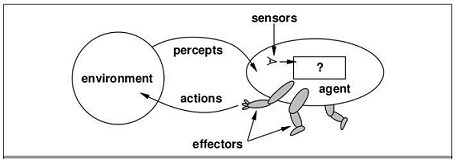
\includegraphics[width=0.6\textwidth]{Imagen2}
\end{center}
\begin{center}
\vskip -0.5cm
\caption{\small{Estructura básica de un agente.}}
{\small{Fuente: \cite{Russel}}}
\end{center}
\end{figure}


\vskip 3cm

\subsection{Estructura de un agente}

Un agente tiene generalmente una estructura en la que se identifican 4 elementos: capacidad de percepción, capacidad de acción, objetivos y entorno.

\begin{itemize}
\item[•] {\bf La capacidad de percepción:}
\vskip 0.1cm El término percepción se utiliza en este contexto para indicar que el agente puede recibir entradas en cualquier instante. La secuencia de percepciones de un agente refleja el historial completo de lo que el agente ha recibido. En general, un agente tomará una decisión en un momento dado dependiendo de la secuencia completa de percepciones hasta ese instante. Si se puede especificar qué decisión tomará un agente para cada una de las posibles secuencias de percepciones, entonces se habrá explicado más o menos todo lo que se puede decir de un agente.

\item[•] {\bf La capacidad de acción:}
\vskip 0.1cm En términos matemáticos se puede decir que el comportamiento del agente viene dado por la función del agente que proyecta una percepción dada en una acción. La función que describe el comportamiento de un agente se puede presentar en forma de tabla; en la mayoría de los casos esta tabla sería muy grande (infinita a menos que se limite el tamaño de la secuencia de percepciones que se quiera considerar). Dado un agente, con el que se quiera experimentar, se puede, en principio, construir esta tabla teniendo en cuenta todas las secuencias de percepción y determinando qué acción lleva a cabo el agente en respuesta. La tabla es, por supuesto, una caracterización externa del agente. 

\begin{table}[ht!]
\centering
\caption{Ejemplo de función de un agente aspiradora.} \vskip 0.1cm
\begin{tabular}{|l|l|}  \hline 
Percept sequence & Action \\ \hline 
\it [A, Clean] & \it Right \\ \it [A, Dirty] & \it Suck \\ \it [B, Clean] & \it Left \\ \it [B, Dirty] & \it Suck \\ \it [A, Clean], \it [A, Clean] & \it Right \\ \it [A, Clean], \it [A, Dirty] & \it Suck \\ \vdots & \vdots \\ \it [A, Clean], \it[A, Clean], \it[A, Clean] & \it Right \\ \it [A, Clean], \it[A, Clean], \it[A, Dirty] & \it Suck \\ \vdots & \vdots \\ \hline
\end{tabular} 
\begin{center}
{\small{Fuente: \cite{Russel}}}
\end{center}
\end{table}

Inicialmente, la función del agente para un agente artificial se implementará mediante el programa del agente. Es importante diferenciar estas dos ideas. La función del agente es una descripción matemática abstracta; el programa del agente es una implementación completa, que se ejecuta sobre la arquitectura del agente. 
\vskip 0.1cm

En general, la arquitectura pone al alcance del programa las percepciones obtenidas mediante los sen­sores, lo ejecuta y alimenta al efector con las acciones elegidas por el programa conforme éstas se van generando. La relación entre agentes, arquitectura y programas podría resumirse de la siguiente manera:
\vskip 0.1cm

\begin{center}
{\bf Agente = Arquitectura + Programa}
\end{center}

Obviamente, el programa que se elija tiene que ser apropiado para la arquitectura. Si el programa tiene que recomendar acciones como Caminar, la arquitectura tiene que tener piernas. La arquitectura puede ser un PC común, o puede ser un coche robotizado con varios computadores, cámaras, y otros sensores a bordo. En general, la arquitectura hace que las percepciones de los sensores estén disponibles para el programa, ejecuta los programas, y se encarga de que los actuadores pongan en marcha las acciones generadas. (Russel)

\item[•] {\bf Los objetivos:}
\vskip 0.1cm Son la esencia del agente. El comportamiento del mismo irá orientado a la consecución de los mismos. Es lo que espera alcanzar el agente después de percibir y actuar según las percepciones para alcanzar dichos objetivos. 

\item[•] {\bf El entorno:}
\vskip 0.1cm Es una característica externa al agente pero que condiciona su comportamiento. Puede ser un mundo tridimensional o una abstracción del mismo reducida a eventos. En otros casos puede ser una matriz la que modele el entorno o incluso un grafo que represente una topología concreta.

\end{itemize}

{\bf Especificación del entorno de trabajo:}
 
Para empezar a diseñar el agente debemos tener una idea clara de las posibles percepciones, acciones, medida de desempeño a satisfacer y la clase de ambiente en la que el agente estará situado. Por sus siglas en inglés, \cite{Russel} la describe como PEAS (performance, environment, actuators, sensors). 

\begin{table}[ht!]
\centering
\caption{PEAS} \vskip 0.1cm
\begin{tabular}{|p{2.5cm} ||p{3cm} |p{2.9cm} |p{2.8cm} |p{3.3cm}|}  \hline 
\bf Agent Type & \bf Performance Measure & \bf Environment & \bf Actuators & \bf Sensors \\ \hline 
Taxi driver & Safe, fast, legal, comfortable trip, maximize profits & Roads, other traffic, pedestrians, customers & Steering, accelerator, brake, signal, horn, display & Cameras, sonar, speedometer, GPS, odometer, accelerometer, engine sensors, keyboard \\ \hline
\end{tabular} 
\begin{center}
{\small{Fuente: \cite{Russel}}}
\end{center}
\end{table}

\subsection{Características}
Las principales características que podemos observar que  posee un agente inteligente se presentan a continuación:

\begin{itemize}
\item[•] {\bf Autonomía:} Los agentes deben trabajar sin supervisión humana, al contrario que los programas que operan en base a interfaces de manipulación directa por parte del usuario. Así, una vez fijadas las condiciones y restricciones necesarias por parte del usuario, se espera que el agente intente cubrir o conseguir sus objetivos, dejando ocultos los detalles para dicho usuario.

\item[•] {\bf Reactividad:} Los agentes deben ser capaces de detectar cambios en su entorno y en consecuencia tomar sus propias decisiones para reaccionar ante ellos.

\item[•] {\bf Adaptabilidad:} Dado a que los agentes reaccionan a los cambios producidos por el entorno, estos provocan que los agentes continuamente aprendan de estas experiencias y se adapten a dichos cambios.

\item[•] {\bf Comunicación:} El agente tiene que tener la capacidad de comunicarse por medio de un lenguaje común con otros agentes de su medio y con los usuarios que interactúa.

\item[•] {\bf Iniciativa o proactividad:} el agente tiene un propósito u objetivo determinado y emprende las acciones necesarias hasta conseguirlo.

\item[•] {\bf Continuidad temporal:} los agentes no sólo realizan ejecuciones en un momento determinado sino que, desde su creación, pasan a un estado de espera hasta cualquier evento provocado por otro agente o usuario, o cualquier cambio producido en el entorno les haga reaccionar. 

\item[•] {\bf Capacidad de proceso:} es capaz de descomponer las consultas en subconsultas y asociar los términos resultantes de esta operación con otros afines.

\item[•] {\bf Conocimiento del entorno donde se mueve:} un agente debe saber en todo momento a qué información acceder o a qué otro agente dirigirse para obtener esta información.

\end{itemize}

\subsection{Clasificación}
Existen multitud de clasificaciones de agentes inteligentes dependiendo del contexto en el que se ubiquen.

\subsubsection{Tipos de Agente Inteligentes}

Según \cite{Russel} los tipos de agentes inteligentes son: 

\begin{itemize}
\item[•] {\bf Agentes de Reflejos Simples} \vskip 0.1cm
Un agente reflejo simple actúa encontrando una regla cuya condición coincida con la situación actual (definida por la percepción) y efectuando la acción que corresponda a tal regla. Sólo funcionará si se toma la decisión adecuada con base en la percepción de un momento dado.

\begin{figure}[ht]
\begin{center}
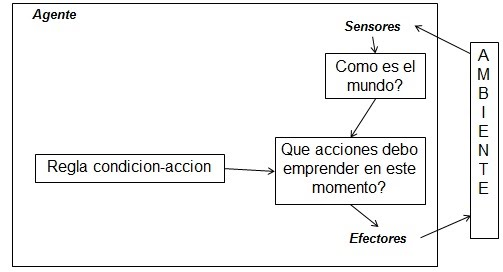
\includegraphics[width=0.6\textwidth]{Imagen3}
\end{center}
\begin{center}
\vskip -0.5cm
\caption{\small{Diseño de Agente de reflejo simple.}}
{\small{Fuente: \cite{Russel}}}
\end{center}
\end{figure}

\vskip 1cm

\item[•] {\bf Agentes Basado en Estado} \vskip 0.1cm
El estado interno le da al agente las condiciones de optar por una acción, este estado actualiza la información, y para ello exige dos conocimientos en el programa de agente.
\begin{itemize}
\item[•] Primero, se necesita información de cómo está evolucionando el mundo, independientemente del agente. \vskip 0.1cm
\item[•] Segundo, se debe informar como las acciones del agente afectan al mundo.
\end{itemize}

Se combina las percepciones prevalecientes con el estado interno anterior para generar la descripción actualizada del estado prevaleciente. En el programa se crea una nueva descripción del estado interno.

\begin{figure}[ht]
\begin{center}
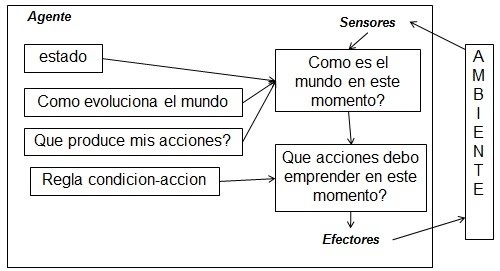
\includegraphics[width=0.6\textwidth]{Imagen4}
\end{center}
\begin{center}
\vskip -0.5cm
\caption{\small{Diseño de agente bien informado de todo lo que pasa.}}
{\small{Fuente: \cite{Russel}}}
\end{center}
\end{figure}

\vskip 1cm
\item[•] {\bf Agentes Basados en Metas} \vskip 0.1cm
Para decidir que hay que hacer, además de una descripción del estado prevaleciente, también se requiere información sobre su meta, información que detalla las situaciones deseables.
\vskip 0.1cm
La búsqueda  y la planificación, son los subcampos de la inteligencia artificial que se ocupa de encontrar las secuencias de acciones que  permiten alcanzar las metas de un  agente. El agente basado en metas es menos eficiente, pero es más flexible.

\begin{figure}[ht]
\begin{center}
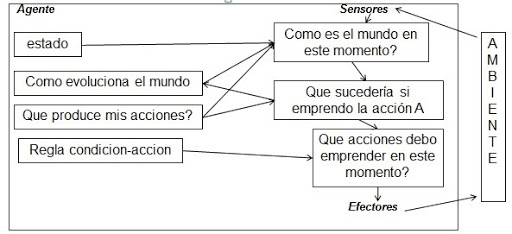
\includegraphics[width=0.7\textwidth]{Imagen5}
\end{center}
\begin{center}
\vskip -0.5cm
\caption{\small{Diseño de agente basado en metas.}}
{\small{Fuente: \cite{Russel}}}
\end{center}
\end{figure}

\vskip 5cm

\item[•] {\bf Agentes Basados en la Utilidad} \vskip 0.1cm
Si se prefiere un estado del mundo por otro, entonces ese estado ofrece mayor utilidad al agente. La utilidad es una función que correlaciona un estado y un número real que corresponde al grado de satisfacción.
\vskip 0.1cm
La utilidad permite la toma de decisiones racionales cuando la meta tiene problemas. Primero, cuando el logro de alguna meta implica un conflicto y sólo alguna de ellas se puede obtener, la utilidad definirá cual es el compromiso adecuado. Segundo, cuando son varias las metas que el agente podría desear obtener, pero no existe la corteza de lograr ninguna de ellas, la utilidad pondera la posibilidad de tener éxito considerando la importancia de las diferentes metas.

\begin{figure}[ht]
\begin{center}
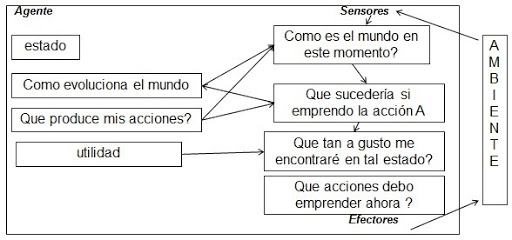
\includegraphics[width=0.7\textwidth]{Imagen6}
\end{center}
\begin{center}
\vskip -0.5cm
\caption{\small{Diseño de agentes basado en utilidades.}}
{\small{Fuente: \cite{Russel}}}
\end{center}
\end{figure}

\end{itemize}

\subsubsection{Clasificación de Agentes según su taxonomía}
\cite{Nwana} nos presenta una clasificación de agentes según su taxonomía:

\begin{figure}[ht]
\begin{center}
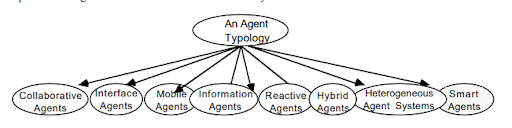
\includegraphics[width=0.9\textwidth]{Imagen7}
\end{center}
\begin{center}
\vskip -0.5cm
\caption{\small{Clasificación de agentes.}}
{\small{Fuente: \cite{Nwana}}}
\end{center}
\end{figure}

\begin{itemize}
\item[•] {\bf Agentes colaborativos o cooperativos:} \vskip 0.1cm
Según {\bf Hípola y Vargas} para que un agente pueda ser autosuficiente y conocedor del entorno en el que se encuentra, debe coordinarse y cooperar con cada uno de los otros agentes. 
\vskip 0.1cm
En un {\bf sistema compartido} un agente cualquiera descompone la consulta y asigna las subconsultas a otros agentes. Cada uno sabe cuáles son las capacidades y limitaciones del resto. No existe un «agente maestro»; el grupo de agentes recibe las subconsultas, y todos ellos trabajan por igual para encontrar la solución.
\vskip 0.1cm
Por el contrario, un {\bf sistema federado} es una estructura jerárquica de agentes controlada por un facilitador o agente principal. Los agentes federados se comunican sólo con su agente principal, el cual conoce las capacidades y limitaciones de cada uno de sus agentes. Una vez recibida la consulta, el facilitador principal se comunica con el resto de facilitadores con el fin de seleccionar los agentes locales más adecuados de cada federación para resolver las subconsultas que permitan resolver la consulta completa.

\item[•] {\bf Agentes de interfaz:} \vskip 0.1cm
Apoyan y dan asistencia, principalmente al usuario, para que aprenda a utilizar una aplicación particular, estos agentes interactúan con el usuario de forma gráfica, de este modo el usuario no tiene porqué conocer todos los procesos que el agente lleva a cabo, sólo los resultados que este le proporciona. 
\vskip 0.1cm
Su objetivo es llevar a cabo búsquedas conceptuales más que localizar simples cadenas de caracteres. Cuando un usuario hace una consulta, la interfaz recoge los términos de ésta como algo representativo de la materia en la que se está interesado. Posteriormente, y a partir de su base de conocimiento, realiza una consulta expandida. Es decir, partiendo de los términos suministrados por el usuario, se añaden otros relacionados con el mismo concepto, realizando así una consulta mucho más completa que la que en un principio se pretendía hacer. Por ejemplo la consulta «perro» puede ser expandida a «perro o can o sabueso».

\item[•] {\bf Agentes móviles:} \vskip 0.1cm
Es uno de los últimos desarrollos en tecnología de agentes. Se basan en el principio organizador de redes de comunicación entre ordenadores, conocido como Control de Procedimientos Remotos (RPC) y concebido en 1976. Cuando un ordenador cliente de una red (no importa su tamaño) dirige una petición al servidor de ficheros para ejecutar una aplicación, el cliente debe realizar al menos dos comunicaciones: una solicitando la ejecución de un programa determinado, y otra informando al servidor que la operación se ha completado con éxito.
\vskip 0.1cm
La alternativa a este procedimiento es la Programación Remota (RP), consistente en acordar por adelantado qué tareas pueden realizar los clientes sin ningún tipo de verificación ni confirmación por parte de los servidores. De esta forma un cliente enviaría una instrucción al servidor de ficheros, y una vez allí ejecutará un programa en concreto. Este procedimiento (remoto) que es una orden realizada por el cliente pero ejecutada en el servidor (local) recibe el nombre de operación o instrucción móvil, haciendo hincapié en que se trata de una orden remota que se ejecuta localmente.
\vskip 0.1cm
Un agente móvil puede suspender el proceso que esté realizando, transportarse a sí mismo por medio de la Red y reanudar la ejecución del proceso que estaba llevando a cabo donde estime oportuno. Esta capacidad le permite al agente seleccionar la información recuperada antes de enviarla por la Red, lo que evita la transferencia de grandes cantidades de información que podría ser inútil.

\item[•] {\bf Agentes de información:} \vskip 0.1cm
Esta tecnología surge como respuesta de los retos que plantea la recuperación de la información en la WWW. Estos agentes cumplen con el papel del manejo, de la manipulación o la recopilación de la información que se encuentran en diferentes fuentes distribuida para dar una respuesta relevante a las cuestiones planteadas por el usuario.

\item[•] {\bf Agentes reactivos:} \vskip 0.1cm
Los agentes reactivos representan una categoría especial de agentes que no poseen modelos internos y simbólicos de sus entornos; en su lugar, actúan / responden en una forma de estímulo-respuesta al estado actual del entorno en el que están incrustados. 
\vskip 0.1cm
Podemos tener tres funciones de estos agentes, la primera sería  la "funcionalidad emergente", es decir, la dinámica de la interacción conduce a la complejidad emergente. Por lo tanto, no existe una especificación (o plan) a priori del comportamiento de la configuración de agentes reactivos. En segundo lugar, se trata de la "descomposición de tareas": un agente reactivo se considera una colección de módulos que funcionan de manera autónoma y son responsables de tareas específicas (por ejemplo, detección, control de motores, cálculos, etc.). La comunicación entre los módulos se minimiza y tiene un carácter bastante bajo. No existe un modelo global dentro de ninguno de los agentes y, por lo tanto, tiene que surgir el comportamiento global. En tercer lugar, los agentes reactivos tienden a operar en representaciones que están cerca de los datos del sensor en bruto, en contraste con las representaciones simbólicas de alto nivel que abundan en los otros tipos de agentes discutidos hasta ahora.

\item[•] {\bf Agentes híbridos:} \vskip 0.1cm
Estos agentes son la combinación de dos o más filosofías dentro de un agente simple (móvil, interfaz, colaborativo, etc.). De este modo se maximizan las habilidades del agente y se minimizan las deficiencias de los diferentes tipos.

\item[•] {\bf Agentes heterogéneos:} \vskip 0.1cm
Los sistemas de agentes heterogéneos, a diferencia de los sistemas híbridos, se refieren a una configuración integrada de al menos dos o más agentes que pertenecen a dos o más clases de agentes diferentes. Un sistema de agente heterogéneo también puede contener uno o más agentes híbridos.
\vskip 0.1cm
Una vez que los agentes están disponibles, hay dos arquitecturas posibles para elegir: una en la que todos los agentes manejan su propia coordinación u otra en la que los grupos de agentes pueden confiar en programas especiales del sistema para lograr la coordinación. La desventaja de la primera es que la sobrecarga de comunicación no garantiza la escalabilidad, que es un requisito necesario para el futuro de los agentes.

\end{itemize}

\subsubsection{Clasificación según su función)}

 \cite{Carrascosa} clasifica los agentes según su función:

\begin{itemize}
\item[•] {\bf Agentes de búsqueda:} \vskip 0.1cm
En un principio, los sistemas expertos fueron diseñados para ejecutar consultas en una sola e independiente base de datos. La aparición de internet ha propiciado el surgimiento de miles de bases de datos almacenadas en diferentes direcciones.
\vskip 0.1cm
La distribución de la información conduce a la necesidad de crear un sistema descentralizado de recuperación de información, que estará basado en agentes inteligentes, los cuales podrán localizar, recuperar y almacenar las preguntas en un «resultado» para un usuario en concreto.
\vskip 0.1cm
Pero los agentes de información no sólo son útiles para la recuperación de información en bases de datos. Hoy día han evolucionado y se utilizan para realizar búsquedas de información textual en artículos de revistas electrónicas o en las páginas web. Independientemente del tipo de información que se quiera localizar, los agentes de búsqueda pueden diferenciarse por la entidad o persona para la que trabajan: usuarios y/o consultas y/o bases de datos. También se pueden distinguir por su forma de interactuar, es decir, si se relacionan libremente todos los agentes para resolver las consultas, o sólo son unos pocos agentes los que se relacionan entre sí (mediadores o principales).
\vskip 0.1cm
Las ventajas que proporcionan estos agentes son:
\begin{itemize}
\item[•] Facilidad de uso - Cuando el usuario sabe lo que quiere puede obtener más resultados.
\item[•] Asimismo el resultado será más preciso, con menos ruido.
\item[•] Se reduce la sobrecarga que se genera por los procesos de búsqueda.
\end{itemize}

\item[•] {\bf Agentes de filtrado:} \vskip 0.1cm
Agentes que, mediante el borrado de los datos no deseados, se ocupan de la sobreabundancia de información. Este tipo de agente es capaz de almacenar, aprender y manipular las preferencias y gustos de cada usuario, así como sus cambios. La tarea de un agente de filtrado consiste en precisar si un documento es relevante o no para un determinado usuario basándose en el perfil de usuario.

\item[•] {\bf Agentes de monitorización:} \vskip 0.1cm
Agentes encargados de alertar al usuario cuando sucede un determinado evento que le pueda resultar de interés. Los agentes de monitorización se pueden considerar como un software localizado en un determinado servidor que se encarga de descubrir y notificar eventos interesantes especificados previamente por el usuario.

\end{itemize}

\subsection{Aplicaciones}
Los agentes inteligentes gracias a su facilidad de adaptabilidad numerosas aplicaciones basadas en este nuevo paradigma vienen siendo empleadas en infinidad de áreas, como describe \cite{Julian} los agentes inteligentes se pueden emplear en procesos industriales, aplicaciones médicas, aplicaciones comerciales y de entretenimiento.
\vskip 0.1cm
Dentro del marco de las aplicaciones industriales podríamos destacar aquellas que se encargan de:

\begin{itemize}
\item[•] {\bf Control de procesos:} 
los controladores son por sí mismos sistemas reactivos. Aplicado a la gestión del transporte de electricidad (ARCHON en el norte de España), control de un acelerador de partículas, monitorización y diagnóstico de fallos en plantas nucleares y control en el proceso de bobinado del acero.

\item[•] {\bf Producción:} 
se ha aplicado con éxito por ejemplo a sistemas encargados de las fases de ensamblaje, pintado, almacenamiento de productos, etc.\vskip 0.1cm
\item[•] {\bf Control de tráfico aéreo:} 
se han desarrollado aplicaciones para el control del tráfico aéreo en aeropuertos como el de Sidney en Australia (OASIS).
\end{itemize}

Otra área de interés son las aplicaciones médicas como por ejemplo:

\begin{itemize}
\item[•] {\bf Monitorización de pacientes en cuidados intensivos:}
empleado para monitorizar y controlar a pacientes ingresados en unidades de cuidados intensivos.
\item[•] {\bf Atención al paciente:}
estos sistemas se encargaría de seguir el tratamiento de un paciente controlando todos los aspectos relativos a la enfermedad que tenga el mismo.
\end{itemize}

También está siendo empleado en aplicaciones comerciales para:

\begin{itemize}
\item[•] {\bf Gestión de información:} 
como por ejemplo el filtrado inteligente de correo electrónico, de grupos de noticias o la recopilación automática de información disponible en la red.

\item[•] {\bf Comercio electrónico:} 
se emplea para proporcionar el entorno virtual donde realizar las operaciones comerciales (compra-venta de productos) o también para realizar tareas de búsqueda de productos (comparando precios, consultando disponibilidad) todo ello de manera automatizada.
\end{itemize}

Por último, también se viene empleando en áreas de entretenimiento como pueden ser:

\begin{itemize}
\item[•] {\bf Juegos:} 
la aplicación de esta tecnología en juegos permite disponer de juegos más sofisticados, con características inteligentes donde se pueden incorporar personajes virtuales que pueden funcionar de forma casi autónoma.

\item[•] {\bf Teatro interactivo y cine:} 
se permite a un usuario interpretar el papel de un personaje en una obra donde el resto de los personajes pueden ser virtuales.
\end{itemize}

\section{Expresiones faciales}

En 1991 un psicólogo llamado Izard quiso cuantificar de alguna forma las diferentes emociones que podía sentir el ser humano. Empezó creando una lista con los diferentes requisitos que debían cumplir las emociones para ser consideradas como básicas:

\begin{itemize}
\item[•] Tener un sustrato neural específico y distintivo.
\item[•] Tener una expresión o configuración facial específica y distintiva.
\item[•] Poseer sentimientos específicos distintivos.
\item[•] Derivar de procesos biológicos evolutivos.
\item[•] Manifestar propiedades motivacionales y organizativas de funciones adaptativas.
\end{itemize}

Con todo esto Izard llegó a la conclusión de que había 8 emociones que cumplían con cada uno de los requisitos anteriores (Placer, interés, sorpresa, tristeza, ira, asco, miedo y desprecio). Pero finalmente fue Ekman, otro de los autores relevantes en el estudio de la emoción quien determinó según los requisitos anteriores 6 emociones básicas: ira, alegría, asco, tristeza, sorpresa y miedo.
\vskip 0.1cm
Mucho antes de que en los años 90 estos psicólogos determinarán las características que diferencian cada emoción, otros intelectuales también repararon en el origen genético de algunas expresiones faciales.
\vskip 0.1cm
Aristóteles dijo “Hay expresiones de la cara características que son observables para acompañar la cólera el miedo, la excitación erótica y todas otras pasiones”.
En el siglo XIX fueron Darwin y Guillaume Duchenne, posteriormente Silvan Tomkis en el siglo XX, hasta que llegó Paul Ekman \citep{Bartual}.
\vskip 0.1cm
Para Ekman la expresión facial es, junto con la mirada, el medio más rico e importante para expresar emociones y estados de ánimo. A través del conocimiento y de la observación de las expresiones faciales (es decir, la cara en movimiento y no como un objeto estático) podemos conseguir una mejor comprensión de lo que nos comunican los demás. Además de manifestar las emociones, la expresión facial se usa principalmente para:  Regular la interacción y reforzar al receptor.
\vskip 0.1cm
Las emociones principales son siete: la tristeza, la ira, la sorpresa, el miedo, el asco, el desprecio y la alegría. La mayor contribución de Ekman en el estudio de las emociones fue demostrar a través de estudios muy completos y muchas fotografías que el rostro de las emociones es universal y se refleja de forma muy similar en cualquier cultura y raza \citep{Ekman}.

\begin{figure}[ht]
\begin{center}
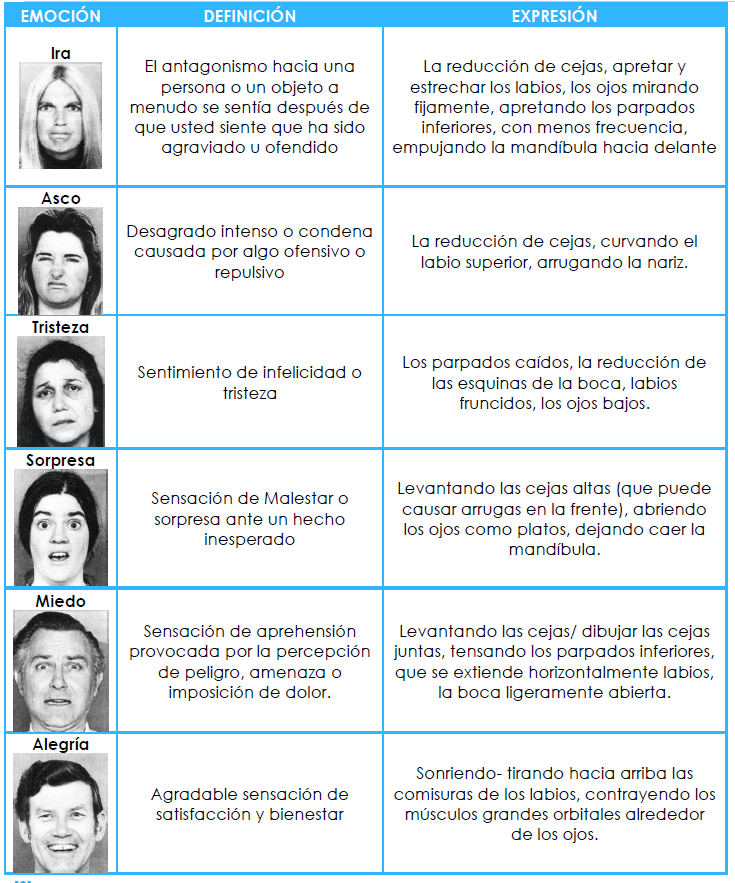
\includegraphics[width=0.55\textwidth]{Imagen8}
\end{center}
\begin{center}
\vskip -0.5cm
\caption{\small{Expresiones faciales según Ekman.}}
{\small{Fuente: \cite{Ekman}}}
\end{center}
\end{figure}

\vskip 5cm

\section{Reconocimiento de expresiones faciales}

El reconocimiento de expresiones faciales es un área del reconocimiento de patrones que ha sido investigada desde hace varios años. Durante todo este tiempo se han propuesto técnicas diferentes para la resolución de esta tarea, entre las que se pueden mencionar \citep{Rafael}

\begin{itemize}
\item Igualamiento de plantillas
\item Cálculo de eigen caras Características Geométricas
\item Métodos que utilizan redes neuronales
\end{itemize}

Independientemente de la técnica que sea implementada, se utilizan siempre dos conjuntos de datos \citep{Santos}:

\begin{itemize}
\item[•] El primero es utilizado siempre para la etapa de aprendizaje, el cual es llamado conjunto de entrenamiento. Se debe tratar de que los patrones que integran este conjunto sean lo más diferente posible entre sí, y que además, representen al problema, para poder tener un buen porcentaje de generalización.
\item[•] El segundo conjunto de patrones, es llamado conjunto de prueba, y es utilizado en la etapa de reconocimiento.
\item[•] Por último, para reconocer una expresión facial se deben realizar los siguientes pasos generales: \vskip 0.1cm

{\bf La captura o adquisición} es el proceso a través del cual se obtiene una imagen digital utilizando un dispositivo de captura como una cámara digital, video cámara, escáner, satélite, etc.
\vskip 0.1cm
{\bf El pre procesamiento,} su función básica es la de mejorar la imagen de forma que se aumenten las posibilidades de éxito en los procesos posteriores. Incluye técnicas tales como la reducción del ruido, realce del contraste, realce de ciertos detalles, o características de la imagen. 
\vskip 0.1cm
{\bf La segmentación} es el proceso que divide una imagen en objetos que sean de nuestro interés de estudio. 
\vskip 0.1cm
{\bf La descripción} es el proceso que obtiene características convenientes para diferenciar un tipo de objeto de otro, como: la forma, el tamaño, área, etc.
\vskip 0.1cm
{\bf El reconocimiento} es el proceso que identifica los objetos, como por ejemplo: una llave, un tornillo, moneda, coche, etc.
\vskip 0.1cm
{\bf La interpretación} es el proceso que asocia un significado a un conjunto de objetos reconocidos (llaves, tornillos, herramientas, etc.) y trata de emular la cognición.

[4]Jorge Rafael Valvert Gamboa, Métodos y Técnicas de Reconocimiento de Rostros en Imágenes Digitales Bidimensionale

[5] Face Analysis Techniques for Human-Computer Interaction , Dissertations in Interactive Technology, Number 8 , Tampere 2017 , University of Tampere 
 
\end{itemize}

\subsection{Captura o adquisición de imágenes}
{\bf Cámara:} \vskip 0.1cm
La cámara es el dispositivo que, utilizando un objetivo formado por un juego de lentes y el diafragma, construye una imagen sobre el plano del sensor compuesto de elementos fotosensibles, la digitaliza y la transmite hacia la tarjeta de adquisición del procesador. Están compuestas por un sensor y la electrónica asociada. Las cámaras proporcionan una señal de vídeo en un formato estándar para su digitalización (en el caso analógico) o directamente la información en formato digital que constituye la imagen captada por la misma \citep{Enrique}.
\vskip 0.1cm


\begin{itemize}
\item[•] {\bf Resolución} \vskip 0.1cm
Es el grado de detalle o calidad de una imagen digital ya sea escaneada, fotografiada o impresa. Este valor se expresa en ppp (píxeles por pulgada) o en inglés dpi (dots per inch). Cuantos más píxeles contenga una imagen por pulgada lineal, mayor calidad tendrá.
\vskip 0.1cm


\item[•] {\bf fps (Fotogramas por segundo)} \vskip 0.1cm
Un video resulta de la exposición imágenes o fotogramas uno detrás de otro. Un parámetro de la calidad del video es el número de fotogramas por segundo que muestra durante su reproducción. Este valor oscila entre 15 y 30.
\vskip 0.1cm

\item[•] {\bf Resolución de la imagen} \vskip 0.1cm
Las cámaras digitales presentan una calidad que se expresa en MegaPíxels. Así por ejemplo una cámara de 8 MP es aquella capaz de tomar una fotografía con 8 millones de píxeles \citep{Web}. 
\vskip 0.1cm


\item[•] {\bf Zoom Digital} \vskip 0.1cm
El zoom digital amplía la imagen que ha recibido reduciendo la resolución. Hará falta que nos fijemos en el tipo de zoom para evaluar la calidad de la cámara. El zoom de una cámara puede venir expresado por el zoom total, que se obtiene de multiplicar el zoom óptico por el digital. Así, por ejemplo, una cámara con zoom óptico 3X (donde X representa el factor de acercamiento, es decir, los aumentos) y zoom digital 8X, tiene un zoom total de 24X \cite{Foto}.
\vskip 0.1cm
\end{itemize}

Para la captura de las secuencias dinámicas de imágenes utilizaremos una cámara Web para poder procesar de inmediato las secuencias a la máquina y poder realizar el procesamiento de las imágenes. 
\vskip 0.1cm
En el mercado podemos encontrar muchos modelos cámaras web con diferentes características, para la presente tesis utilizaremos una cámara de gama media, a continuación presentamos algunas de las más comunes.

\begin{enumerate}
{\bf\item[1. ] Microsoft LifeCam HD-3000} \vskip 0.1cm
Es una buena cámara de chat de vídeo pero no es tan completa como los modelos mejor clasificados, pero cumple con las especificaciones para grabar en buena calidad.
\begin{itemize}
\item[•] {\bf Resolución video:}
1280 x 720 píxeles
\item[•] {\bf fps:}
30
\item[•] {\bf Resolución imagen:}
1 MP
\item[•] {\bf Zoom digital:}
4X
\end{itemize}

\begin{figure}[ht]
\begin{center}
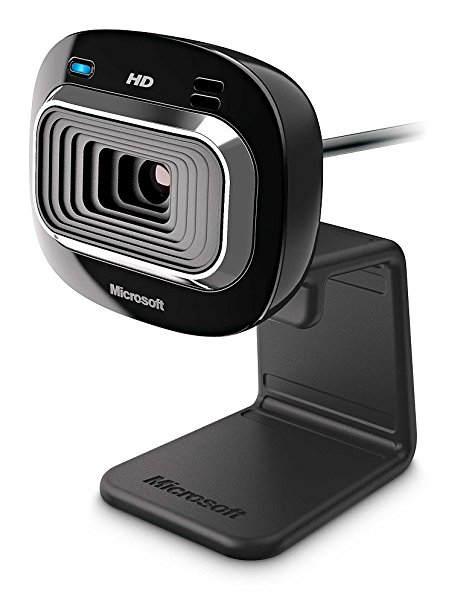
\includegraphics[width=0.2\textwidth]{Imagen9}
\end{center}
\begin{center}
\vskip -0.5cm
\caption{\small{Microsoft LifeCam HD-3000}}
{\small{Fuente: \cite{Amazon}}}
\end{center}
\end{figure}

{\bf\item[2. ] Hd Logitech C270} \vskip 0.1cm
Logitech C270 es una cámara web de escritorio con una gran calidad de imagen. Videoconferencias HD con el sistema recomendado. Fotos: Hasta 3.0 megapíxeles.
\begin{itemize}
\item[•] {\bf Resolución video:}
1280 x 720 píxeles
\item[•] {\bf fps:}
30
\item[•] {\bf Resolución imagen:}
4 MP
\item[•] {\bf Zoom digital:}
4X
\end{itemize}

\begin{figure}[ht]
\begin{center}
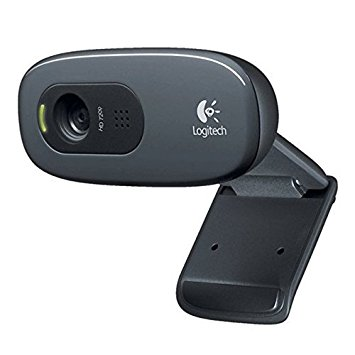
\includegraphics[width=0.2\textwidth]{Imagen10}
\end{center}
\begin{center}
\vskip -0.5cm
\caption{\small{Hd Logitech C270}}
{\small{Fuente: \cite{Amazon}}}
\end{center}
\end{figure}

{\bf\item[3. ] Genius FaceCam 1000X} \vskip 0.1cm
Cuenta con un diseño simple de clip, con lo cual se adapta fácil a cualquier pantalla u ordenador.
\begin{itemize}
\item[•] {\bf Resolución video:}
1280 x 720 píxeles
\item[•] {\bf fps:}
30
\item[•] {\bf Resolución imagen:}
3 MP
\item[•] {\bf Zoom digital:}
3X
\end{itemize}

\begin{figure}[ht]
\begin{center}
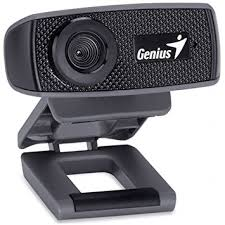
\includegraphics[width=0.15\textwidth]{Imagen11}
\end{center}
\begin{center}
\vskip -0.5cm
\caption{\small{Genius FaceCam 1000X.}}
{\small{Fuente: \cite{Amazon}}}
\end{center}
\end{figure}

\end{enumerate}
\vskip 1cm

\subsection{Pre procesamiento de la imagen}
Como se puede intuir las imágenes de una misma persona son captadas de una secuencia de imágenes en momentos diferentes, lo que conlleva a que cada imagen sea diferente, debido a que puede variar la iluminación, el ángulo de enfoque y el tamaño del rostro (profundidad). Por esto es necesario pre procesar la imagen. Entre las tareas más comunes de pre procesamiento se puede mencionar:

\begin{enumerate}
{\bf\item[A. ] Técnicas de realce} \vskip 0.1cm
La gran mayoría de imágenes de expresión facial tienen un pobre contraste. Es por esto que es necesario realzar el contraste de estas imágenes antes de un procesamiento posterior o de realizar un análisis. Existen diferentes técnicas para realzar el contraste, entre las cuales se tienen:

\begin{itemize}
{\bf \item[•] Ampliación del contraste} \vskip 0.1cm
La idea de esta técnica es aumentar el valor de intensidad minimo y maximo de los niveles de gris de una imagen. La manipulación clásica de contraste se basa en una ampliación definida globalmente, esta función(figura 2.11 (a)) se define por un perfil de transformación elegido de forma apropiada para lograr el incremento de contraste deseado \citep{Zeyun}. 
\vskip 0.1cm
Una forma general de transformación se muestra en la ecuación 2.1, en donde Si son los valores que separan los diferentes modos del histograma y L es el valor de nivel de gris máximo. 

\begin{equation}
f(x)= \left\{ \begin{array}{lcc}
             f_{1}(x), & & 0 \leqslant x \leqslant S_{1}  \\
             \\ f_{2}(x), & & S_{1} \leqslant x \leqslant S_{2} \\
             \\ & \vdots & \\
             \\ f_{n}(x), & & S_{n-1} \leqslant x \leqslant L 
             \end{array}
   \right.
\end{equation}

\vskip 0.1cm 
Difiere de la ecualización del histograma en que solo puede aplicarse una función escalado lineal a los valores de los píxeles de la imagen.

\begin{figure}[ht]
\begin{center}
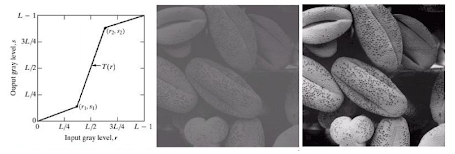
\includegraphics[width=0.7\textwidth]{Imagen12}
\end{center}
\begin{center}
\vskip -0.5cm
\caption{\small{Aumento del contraste (a) función de transformación (b) imagen con bajo contraste (c) resultado de aumento del contraste.}}
{\small{Fuente: \cite{Zeyun}}}
\end{center}
\end{figure}

{\bf \item[•] Ecualización por Histograma} \vskip 0.1cm
La ecualización del histograma se basa en lograr una distribución más uniforme entre el número de píxeles referido con respecto a los diferentes niveles de intensidad (NI) que presenta en la imagen. Su función radica en aumentar y disminuir al mismo tiempo el contraste de la imagen, mediante el incremento y reducción de los NI que se encuentran más cercanos al valor máximo y mínimo del histograma respectivamente. Matemáticamente la ecualización del histograma H(Q) se define como \citep{Pajares}

\begin{equation}
H(Q)=\frac{L-1}{n*m} 
\displaystyle\sum_{j=0}^{Q} h_f (j)
\end{equation}

Donde Donde L es el valor máximo del conjunto Q= {0, ..., Q - 1} que representa los q Niveles de Intensidad (NI) de la imagen f: n x m $\rightarrow$ Q x Q con dimensión de (n x m) y donde hf es el histograma de la imagen. \vskip 0.1cm
Debido a la redistribución de esta probabilidad de ocurrencia de niveles de grises de una manera uniforme, la percepción de los detalles de la imagen mejora. De la ecuación anterior se pueden derivar diferentes tipos de ecualizaciones, siendo las más conocidas ecualización uniforme, exponencial y la de Rayleigh \citep{Pajares}. \vskip 0.1cm
[6] PAJARES MARTÍ SANZ, Arturo y DE LA CRUZ, Jesús M. Visión por computador, imágenes digitales y aplicaciones. España, 2001.

{\bf \item[•] Filtro paso alto} \vskip 0.1cm
Según \citep{Enrique} los filtros paso alto realizan un realzado de los detalles de la imagen. Este tipo de filtros atenúa las zonas uniformes y enfatiza los detalles de interés. Al contrario que los filtros paso bajo, elimina el componente media. Permitir el paso de las altas frecuencias produce como resultado una imagen llena de bordes y discontinuidades en la que la eliminación de los términos de baja frecuencia produce una reducción significativa del contraste global de la imagen. Debe tener coeficientes negativos en la periferia y positivos en el centro, y la suma de todos ellos debe ser cero. Así, cuando la máscara se encuentre sobre una zona uniforme, la salida proporcionada por la máscara será cero o próxima a dicho valor (Figura 2.12).

\begin{figure}[ht]
\begin{center}
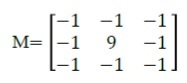
\includegraphics[width=0.25\textwidth]{Imagen13}
\end{center}
\begin{center}
\vskip -0.5cm
\caption{\small{Máscara de convolución de 3x3 Kernel.}}
{\small{Fuente: \cite{Enrique}}}
\end{center}
\end{figure}

{\bf\item[B. ] Técnicas de reducción de ruido mediante filtros} \vskip 0.1cm
El ruido es información no deseada que contamina la imagen. Este aparece durante el proceso de adquisición y digitalización, haciendo necesario implementar un método de reducción de ruido, que retenga tanto como sea posible las características de importancia. Existen diferentes técnicas para la reducción de ruido:

\begin{enumerate}
{\bf\item[B.1. ] Apertura:}
pretende eliminar algunas zonas de los píxeles del frente, siendo en general menos destructiva que la erosión. Se utiliza para eliminar ruido de las imágenes. Es una combinación de las dos operaciones morfológicas básicas: APERTURA = EROSIÓN + DILATACIÓN.

\begin{figure}[ht]
\begin{center}
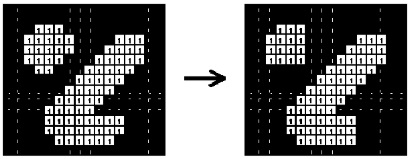
\includegraphics[width=0.6\textwidth]{Imagen14}
\end{center}
\begin{center}
\vskip -0.5cm
\caption{\small{Imagen aplicada apertura.}}
{\small{Fuente: \cite{Matlab}}}
\end{center}
\end{figure}

\begin{enumerate}
{\bf\item[B.1.1. ] EROSIÓN:}
se superpone un kernel por todos los elementos del primer plano (valor 1) y si alguno se superpone a uno que valía 0, el elemento central pasará a valer 0. \citep{Matlab}

\begin{figure}[ht]
\begin{center}
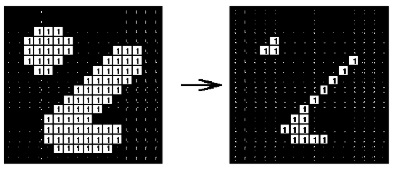
\includegraphics[width=0.6\textwidth]{Imagen15}
\end{center}
\begin{center}
\vskip -0.5cm
\caption{\small{Imagen aplicada erosión.}}
{\small{Fuente: \cite{Matlab}}}
\end{center}
\end{figure}

{\bf\item[B.1.2. ] DILATACIÓN:}
se pasa por los píxeles del fondo. Al superponerla por todos los elementos del fondo (por todos los 0), si está sobre algún píxel que valga 1, se pone el central también a 1. \citep{Matlab}

\begin{figure}[ht]
\begin{center}
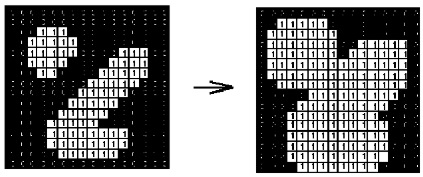
\includegraphics[width=0.6\textwidth]{Imagen16}
\end{center}
\begin{center}
\vskip -0.5cm
\caption{\small{Imagen aplicada dilatación.}}
{\small{Fuente: \cite{Matlab}}}
\end{center}
\end{figure}

\end{enumerate}

\vskip 1cm
{\bf\item[B.2. ] Filtrado de mediana:}
reduce el ruido en una imagen de una forma parecida a como lo hace el filtro de la media. Suele dar mejor resultado al preservar algunos detalles útiles de la imagen. El procedimiento es el siguiente: se toma el píxel y ocho vecinos - kernely se reemplaza el valor del píxel por la mediana de los valores. Para calcular la mediana se ordenan los píxeles en orden ascendente o descendente tomándose el valor del medio (valor 5). Si el entorno que se estudia contiene un número par de píxeles, se toma la mediana como la media aritmética de los dos valores centrales \citep{Matlab}.

\begin{figure}[ht]
\begin{center}
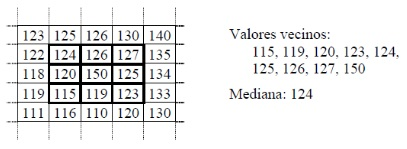
\includegraphics[width=0.6\textwidth]{Imagen17}
\end{center}
\begin{center}
\vskip -0.5cm
\caption{\small{Filtro de la mediana con máscara 3x3.}}
{\small{Fuente: \cite{Matlab}}}
\end{center}
\end{figure}

{\bf\item[B.3. ] Filtro Gaussiano:}
el kernel utilizado en este tipo de filtros contiene como coeficientes valores que siguen una distribución Gaussiana bivariante. Si la media y la varianza son las mismas para los dos ejes los valores pueden ser obtenidos mediante:

\begin{equation}
G(x,y)=\frac{1}{\sigma^2}{e^{-\frac{x^2+y^2}{2\sigma^2}}}
\end{equation}

Donde $\sigma$ es la desviación estándar de la distribución. En la siguiente figura se da el ejemplo de una máscara de 5x5 para el filtro gaussiano con $\sigma$ = 1.0 
\vskip 0.1cm
El valor máximo aparece en el píxel de referencia y disminuye en función de la varianza establecida $\sigma$!. Por tanto, la contribución de cada píxel al valor final disminuye con la distancia. En la práctica, este tipo de filtros se utilizada como etapa de preprocesado para la detección de bordes u otras operaciones \citep{Enrique}.

\end{enumerate}

\end{itemize}
\end{enumerate}

\subsection{Segmentación}
Cuando la imagen es mejorada pasa por un proceso de segmentación para aislar el rostro de la persona del resto de la imagen. Con la cara aislada, el sistema se enfoca en ubicar las posiciones de los gestos faciales con el objetivo de utilizar estas posiciones en el recorte de la imagen del rostro. Si esto no se logra para la imagen de entrada, el sistema tiene gran probabilidad de fallar en su reconocimiento.

\subsubsection{Descriptor Haar}
El esquema de detección de objetos propuesto por Viola \& Jones usando características de tipo Haar es uno de los algoritmos basados en AdaBoost más populares y de alto rendimiento. El mismo ha sido utilizado en la detección de rostros, detección de peatones y la detección de coches \citep{Fernando}.
\vskip 0.1cm
Un detector de objetos basado en descriptores tipo Haar toma principalmente tres tipos de filtros digitales, para detectar orillas, líneas y diagonales. El valor de una característica de dos rectángulos es la diferencia entre la suma de los píxeles dentro de las dos regiones. Estas regiones tienen el mismo tamaño y la misma forma y son adyacentes vertical u horizontalmente. Una característica de tres rectángulos calcula la suma dentro de los rectángulos de las orillas y lo resta de la suma del rectángulo del centro. Finalmente una característica basada en cuatro rectángulos calcula la diferencia entre los pares diagonales de los rectángulos (figura 2.17) \citep{Lopez}.

\begin{figure}[ht]
\begin{center}
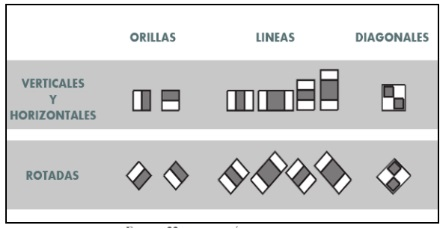
\includegraphics[width=0.5\textwidth]{Imagen18}
\end{center}
\begin{center}
\vskip -0.5cm
\caption{\small{Características de Haar.}}
{\small{Fuente: \cite{Lopez}}}
\end{center}
\end{figure}

\subsubsection{Descriptor HOG (Histograma de Gradiente Orientado)}
El método Histograma de Gradiente Orientado (HOG), propuesta por , se aplica para la detección humana. La idea básica de HOG se basa en que la observación en la apariencia local del objeto y la forma, pueden a menudo caracterizarse bastante bien por la distribución de los gradientes de intensidad locales o direcciones de bordes. Las características de HOG se derivan en base a una serie de orientaciones locales de histogramas de gradiente de la imagen bien normalizados en una densa red. En particular, la imagen se divide en pequeñas celdas. Para cada celda, un histograma local del gradiente, direcciones u orientaciones de borde, se acumula sobre los píxeles de la celda. Todos los histogramas dentro de las celdas de un bloque se normalizan para reducir el efecto de la variación de iluminación. Los bloques se pueden superponer entre sí para mejorar el rendimiento. Las características finales del HOG se forman mediante la concatenación de todos los histogramas normalizados en un único vector. A continuación se muestra en detalle el algoritmo del descriptor local HOG \citep{Aguilar}.

\begin{itemize}
\item[•] Paso 1: Calcular el gradiente horizontal y vertical de la imagen de entrada mediante la convolución con una máscara derivativa.
\item[•] Paso 2: Calcular la magnitud y la orientación del gradiente. Gh y Gv denotan el gradiente horizontal y el vertical, respectivamente. La magnitud del gradiente Ng y la orientación Og en el punto (x, y) son calculados como sigue:

\begin{equation}
N_{g}(x,y)=\sqrt{G_{h}(x,y)^2+G_{v}(x,y)^2} 
\end{equation}

\begin{equation}
O_{g}=arctan(\frac{G_{h}(x,y)}{G_{v}(x,y)})
\end{equation}

\item[•] Paso 3: Dividir la imagen en celdas. Calcule el histograma para cada celda. Suponiendo que el histograma se divide en K contenedores basado sobre la orientación, el valor del i-ésimo contenedor Vi para la celda C se calcula de la siguiente manera:

\begin{equation}
V_{i}=\sum_{(x,y)\in C} \{ {N_g(x,y), O_g(x,y)\in Bin_i} \}
\end{equation}

\item[•] Paso 4: Normalizar todos los histogramas de las celdas dentro un bloque.
\item[•] Paso 5: Concatenar todos los histogramas normalizados para formar el vector de características HOG.

\begin{figure}[ht]
\begin{center}
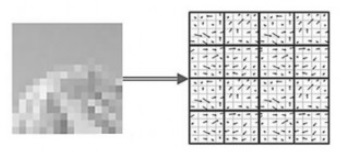
\includegraphics[width=0.4\textwidth]{Imagen19}
\end{center}
\begin{center}
\vskip -0.5cm
\caption{\small{Cálculo de gradientes en esquema HOG.}}
{\small{Fuente: \cite{Fernando}}}
\end{center}
\end{figure}

\end{itemize}

\subsection{Descripción}
A continuación, se presentan algunas de las principales técnicas de descripción de características utilizadas actualmente:

\begin{enumerate}
{\bf\item Análisis de componentes independientes (ICA):} \vskip 0.1cm
El ICA es una generalización de PCA y a diferencia de este el ICA provee una mejor representación de la imagen ya que no se basa únicamente en estadísticas o relaciones entre píxeles de la imagen de segundo orden, sino que es sensible a dependencias estadísticas de alto orden y no solo la covarianza, lo que la hace de ICA una representación potente para las tareas de reconocimiento de rostros y de emociones \citep{Willian}. 
\vskip 0.1cm
El problema que trata de resolver ICA consiste en recuperar un vector que contiene las señales originales independientes a las que se les denomina fuentes S, disponiendo, únicamente, de un vector de observaciones X las cuales son sumas ponderadas de las señales originales \citep{Damian}, mediante la expresión:  S = W * X
\vskip 0.1cm
Para realizar esta tarea es por lo tanto necesario estimar una matriz de pesos W. Para obtener los pesos W, que se usan para obtener las componentes independientes (ICs), se maximiza la negentropía (medida de no Gaussianidad) y de esta forma se consigue minimizar la información mutua entre las señales de entrada. Es importante considerar que la estimación de ICA usando la no Gaussianidad, se puede simplificar haciendo que las observaciones X sean centradas y tengan varianza unitaria. Este preprocesamiento para ICA se consigue en dos pasos: el primero es sustraer de X su vector de media y el segundo es realizar un blanqueamiento de las variables observadas centradas, para esto se calcula una matriz de blanqueamiento dada por \citep{Damian}.

\begin{equation}
W_{z}={2(Cov(X))}^{-\frac{1}{2}}=2(XX^{T})^{-\frac{1}{2}}
\end{equation}

De forma que los datos blanqueados se consiguen como:

\begin{equation}
X_{blanqueado}=W_{z}*X_{centrado}
\end{equation}

El ICA sobre imágenes puede realizarse basándose en dos diferentes arquitecturas (Figura 2), la primera trata la imagen como una señal aleatoria y los píxeles como salidas y una segunda la cual trata los píxeles como variables aleatoria y las imágenes como salidas. La primera arquitectura produce imágenes bases estadísticamente independientes, sin embargo los coeficientes que codifican cada rostro no son necesariamente independientes, por lo que se requiere de una segunda arquitectura que use ICA para encontrar una representación en la cual los coeficientes usados para codificar las imágenes sean estadísticamente independientes \citep{Willian}.

\begin{figure}[ht]
\begin{center}
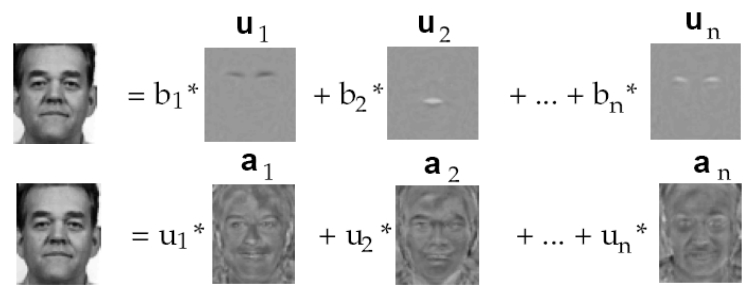
\includegraphics[width=0.6\textwidth]{Imagen20}
\end{center}
\begin{center}
\vskip -0.5cm
\caption{\small{Arquitecturas 1 y 2 de ICA para imágenes.}}
{\small{Fuente: \cite{Willian}}}
\end{center}
\end{figure}

\vskip 3cm

{\bf\item Patrón binario local (LBP):} \vskip 0.1cm
LBP es un simple descriptor de textura propuesto por (Timo Ojala et al., 1996). El operador de textura LBP, que trabaja con un vecindario de 3x3, toma valores de los ocho píxeles vecinos, tomando como umbral para asignación binaria el valor del píxel central. A continuación los valores binarios se ponderan por potencias de dos y se suman para obtener el código LBP del píxel central \citep{Adams}. La Figura 2.20 muestra un ejemplo del operador LBP.

\begin{figure}[ht]
\begin{center}
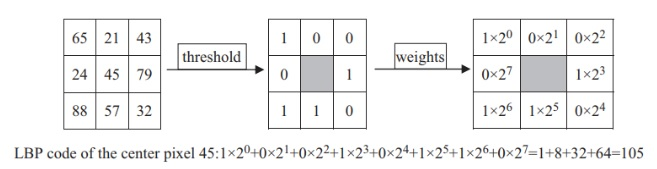
\includegraphics[width=0.8\textwidth]{Imagen21}
\end{center}
\begin{center}
\vskip -0.5cm
\caption{\small{Un ejemplo del operador LBP.}}
{\small{Fuente: \cite{Adams}}}
\end{center}
\end{figure}

Si se definen gc y g0, …., g7  que denotan respectivamente a los valores en escala de grises del centro y de los píxeles del entorno, el código de LBP para el píxel central con coordenadas (x, y) se calcula: 

\begin{equation}
LBP(x,y)=\sum_{p=0}^{7}s(g_{c}-g_{p})*2^{p}
\end{equation}

Donde s(*) es la función de umbral definida como:

\begin{equation}
s(z)= \left\{ \begin{array}{lcc}
             1 & si & z \geqslant 0 \\
             \\ 0 & si & z<0 
             \end{array}
   \right.
\end{equation}

La extensión es capaz de tomar cualquier radio y vecinos alrededor de un píxel central, denotado por LBP(p,r),  mediante el uso de un vecindario circular y la interpolación bilineal cada vez que el punto de muestreo no cae en el centro de un píxel \citep{Adams}. La Figura 2.21 muestra un ejemplo con diferentes vecinos y radios.

\begin{figure}[ht]
\begin{center}
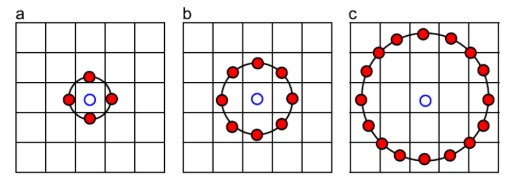
\includegraphics[width=0.6\textwidth]{Imagen22}
\end{center}
\begin{center}
\vskip -0.5cm
\caption{\small{Distintos tipos de vecindarios.}}
{\small{Fuente: \cite{Adams}}}
\end{center}
\end{figure}

En la Figura 2.21 a) se muestra un LBP(4,0) de 4 vecinos y radio 0, en la Figura 2.21 b) se muestra un LBP(8,1) de 8 vecinos y radio 1 y en la Figura 2.21 c) se muestra un LBP(16,2) de 16 vecinos y radio 2 \citep{Adams}.
\vskip 0.1cm
Una vez explicado cómo se aplica el operador LBP en un punto de la imagen, es necesario dar a conocer como se ordena y almacena esta información. En el caso del método LBP el elemento que se obtiene al aplicarlo a una imagen es un vector. Dicho vector es una concatenación de los histogramas que se obtienen al tomar una imagen y subdividirla en ventanas. A cada punto en la ventana se le aplica el operador LBP dándole un valor a cada pixel. Luego se generan los histogramas para cada ventana y finalmente concatenan estos histogramas para dar origen al vector descriptor de la imagen (Ver Figura 2.22). \citep{Adams}. 

\begin{figure}[ht]
\begin{center}
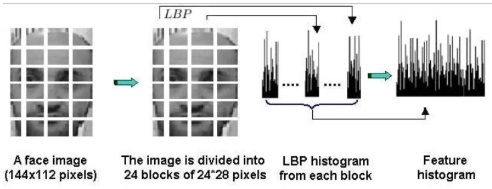
\includegraphics[width=0.6\textwidth]{Imagen23}
\end{center}
\begin{center}
\vskip -0.5cm
\caption{\small{Ilustra el proceso de extracción de características para imágenes de caras.}}
{\small{Fuente: \cite{Aguilar}}}
\end{center}
\end{figure}

{\bf\item Filtro Gabor:} \vskip 0.1cm
El filtro de Gabor, propuesto por Gabor en 1943, se define como el producto de una exponencial compleja por una función gaussiana. Son filtros que tienen como principal característica que, al introducir el envolvente gaussiano, se localizan tanto en el dominio espacial como en el de la frecuencia \citep{Aguilar}. 
\vskip 0.1cm
En el reconocimiento facial las grandes variaciones pueden afectar seriamente al rendimiento de este. Para superar esta degradación del rendimiento, se utilizan los Filtros Gabor, los cuales al ser convolucionados con imágenes faciales extraen lo que se conoce como Características de Gabor, siendo entonces más robustos a distorsiones locales debidas a iluminación o expresión \citep{Adams}.
\vskip 0.1cm
El Filtro de Gabor bidimensional ha sido ampliamente utilizado para reconocimiento facial robusto. La parte real $g_{r}$ y la parte imaginaria de $g_{i}$ del Filtro Gabor se representan como: 

\begin{equation}
g(x, y; \lambda; \sigma; \gamma; \theta; \psi) = g_{r}(x, y; \lambda; \sigma; \gamma; \theta; \psi)+j g_{i}(x, y; \lambda; \sigma; \gamma; \theta; \psi);
\end{equation}

\begin{equation}
g_{r}(x, y; \lambda; \sigma; \gamma; \theta; \psi) = \frac{\gamma}{2\pi\sigma^{2}}exp(-\frac{x_r^2+\gamma^2y_r^2}{2\sigma^2})cos(2\pi\frac{x_{r}}{\lambda}+\psi), 
\end{equation}

\begin{equation}
g_{i}(x, y; \lambda; \sigma; \gamma; \theta; \psi) = \frac{\gamma}{2\pi\sigma^{2}}exp(-\frac{x_r^2+\gamma^2y_r^2}{2\sigma^2})sen(2\pi\frac{x_{r}}{\lambda}+\psi), 
\end{equation}

\begin{equation}
x_{r}=xcos(\theta)+ysen(\theta),
\end{equation}

\begin{equation}
y_{r}=-xsen(\theta)+ycos(\theta),
\end{equation}

Donde $\lambda$ es la longitud de onda de la onda plana sinusoidal de modulación; $\sigma$ es el ancho de la gaussiana envolvente; $\gamma$ es la relación de aspecto espacial; $\theta$ es la orientación del eje mayor de la función elíptica; y $\psi$ es el desplazamiento. Para un determinado filtro de Gabor con valores específicos de $\lambda, \sigma, \gamma, \theta$ y $\psi$, una característica Gabor $f$ correspondiente a una orientación $\theta_{j}$, en una ubicación $(x_{i},y_{i})$ en una imagen $I$, se representa como:

\begin{equation}
f(x_{i},y_{i},\theta_{i})=\sqrt{\{O_{R}(x_{i},y_{i},\theta_{i})\}^{2}+\{O_{I}(x_{i},y_{i},\theta_{i})\}^{2}},
\end{equation}

\begin{equation}
O_{R}(x_{i},y_{i},\theta_{i})=g_{R}(\theta_{j}|\lambda,\sigma,\gamma,\psi)\otimes I(x_{i},y_{i}),
\end{equation}

\begin{equation}
O_{I}(x_{i},y_{i},\theta_{i})=g_{I}(\theta_{j}|\lambda,\sigma,\gamma,\psi)\otimes I(x_{i},y_{i}),
\end{equation}

Donde $\otimes$ denota la operación de convolución en la ubicación $(x_{i},y_{i})$. Se debe tener en cuenta que $f$ contiene sólo la información de la magnitud de $O_{r}$ y $O_{i}$. Dado que hay $N_{o}$ orientaciones para cada una de las $N_{l}$ ubicaciones, entonces un conjunto de filtros de Gabor genera un vector de características Gabor $f$ consiste en $N_{o}xN_{l}$ características Gabor $f$, es decir: 

\begin{equation}
f=[f_{1},...\ ...,f_{N_{0}xN_{l}}]^{T}
\end{equation}

Se debe mencionar que aplicar este método a todos los puntos de una imagen da como resultado un vector de características excesivamente grande, por lo que en estos casos lo que se debe realizar es una selección de puntos de una imagen a utilizar \citep{Adams}.

\begin{figure}[ht]
\begin{center}
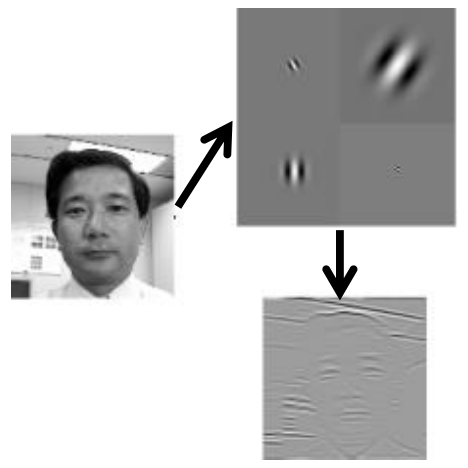
\includegraphics[width=0.6\textwidth]{Imagen24}
\end{center}
\begin{center}
\vskip -0.5cm
\caption{\small{Ilustración de la imagen resultante al aplicar un filtro de Gabor.}}
{\small{Fuente: \cite{Aguilar}}}
\end{center}
\end{figure}

\end{enumerate}

\subsection{Reconocimiento e interpretación}

El reconocimiento e interpretación consiste en alimentar al agente con imágenes de expresiones faciales de rostros diferentes a las utilizadas durante el aprendizaje, esperando obtener como resultado, alguna forma de codificación que nos permita saber de qué persona se trata para ellos se utilizara un clasificador.
\vskip 0.1cm
Podemos entender la clasificación como el proceso de asignar objetos a un conjunto prefijado de categorías o clases. En el caso que nos atañe, estas categorías vienen determinadas por las emociones que queremos detectar a partir de una serie de características medidas sobre los individuos. Cuando conocemos a priori el conjunto de clases (emociones), el proceso de clasificación recibe el nombre de clasificación supervisada.

\begin{enumerate}
{\bf \item Redes Neuronales:} \vskip 0.1cm
El método de aprendizaje conocido como Redes Neuronales fue desarrollado simultáneamente en los ámbitos del análisis estadístico y de la inteligencia artificial. La idea central consiste en extraer combinaciones lineales de los atributos presentes en los objetos obteniendo una serie de características y modelizar las clases como funciones no lineales de dichas características. Karpouzis et al. (1999) y Yacoub et al. (2003) presentan algunos ejemplos de la aplicación de esta técnica de clasificación al problema de reconocimiento de emociones. En el primero de estos artículos, las redes neuronales son adaptadas para identificar y agrupar los músculos de la cara que contribuyen a detectar las emociones. En el segundo artículo las emociones tratan de ser reconocidas a partir de señales obtenidas del discurso. Las redes neuronales obtuvieron mejores resultados de clasificación que las técnicas alternativas con las que son comparadas: máquinas de vectores soporte y k-vecinos más cercanos \citep{Isaac}.

{\bf \item Máquinas de Vector Soporte:} \vskip 0.1cm
Según \citep{Isaac} Las Máquinas de Vectores Soporte (o SVM de ‘Support Vector Machine’) son procedimientos de clasificación y regresión basados en la teoría estadística del aprendizaje. Podemos definir una SVM como una clase específica de algoritmos preparados para el entrenamiento eficaz de una máquina de aprendizaje lineal en un espacio inducido por una función núcleo (o kernel), de acuerdo a unas reglas de generalización empleando técnicas de optimización. Las dos ideas fundamentales para la construcción de un clasificador SVM son la transformación del espacio de entrada en un espacio de alta dimensión y la localización en dicho espacio de un hiperplano separador óptimo. La transformación inicial se realiza mediante la elección de una función kernel adecuada. La ventaja de trabajar en un espacio de alta dimensión radica en que las clases consideradas serán linealmente separables con alta probabilidad, y por tanto, encontrar un hiperplano separador óptimo será poco costoso desde el punto de vista computacional. Además, dicho hiperplano vendrá determinado por unas pocas observaciones, denominadas, vectores soporte por ser las únicas de las que depende la forma del hiperplano. Una de las principales dificultades en la aplicación de este método radica en la elección adecuada de la función kernel. Es decir, construir la función de transformación del espacio original a un espacio de alta dimensión es un punto crucial para el buen funcionamiento del clasificador.
\vskip 0.1cm
En el problema del reconocimiento de emociones es típico trabajar con más de dos emociones. Supongamos que el número de emociones consideradas es n. Es necesario llevar a cabo una generalización del clasificador binario al caso multiclase.
\vskip 0.1cm
Existen varios algoritmos para esta generalización. En primer lugar, el algoritmo de “uno frente a uno”, donde se entrena un clasificador binario por cada par de emociones disponibles. Dispondremos por tanto de 2*n clasificadores, es decir, 2*n valores de la regla de clasificación para cada objeto. El algoritmo “uno frente a todos” supone entrenar tantos clasificadores binarios como número emociones estén disponibles. En este caso disponemos n clasificadores, es decir, n valores de la regla de clasificación para cada objeto. En ambos casos para determinar la emoción que corresponde a cada objeto se realiza una ponderación sobre todas las reglas de clasificación disponibles.
\vskip 0.1cm
Las SVMs han demostrado ser un método muy efectivo en la clasificación de expresiones faciales espontáneas (Bartlett et al., 2001)). Srivastavaa et al. (2006) han empleado con éxito las SVMs con kernel polinomial para el reconocimiento de personas empleando imágenes de rango de los rostros.

{\bf \item k vecinos más próximos (KNN):} \skip 0.1cm
Este algoritmo se basa en la distancia que existe entre la muestra de entrada con las diferentes muestras que se tienen ya clasificadas por clases. Dependiendo del número de vecinos en los que se fije determinará la clase de la muestra. Ésta corresponderá a la clase más dominante entre los K vecinos más próximos \citep{Bartual}. 
\vskip 0.1cm
KNN es un clasificador estadístico basado en el vecino más cercano (KNN), el cual visto de un modo práctico encuentra los k patrones del conjunto de entrenamiento más próximos al patrón observación con una métrica dada (para el caso de este estudio la distancia Euclidiana), anota las clases a las que pertenecen dichos patrones y decide por votación mayoritaria entre las clases de los k patrones \citep{Damian}.
\end{enumerate}

\section{Secuencia dinámica de imágenes}
\subsection{Definición:}
Las escenas dinámicas a menudo incluyen múltiples objetos en movimiento, cada uno de los cuales puede cambiar su estado de movimiento y mostrar un movimiento complicado, algunas aplicaciones trabajan con colecciones de imágenes relacionadas con el tiempo, como fotogramas de una película, o por la localización espacial, como la resonancia magnética nuclear (RMN). Estas colecciones de imágenes se conocen como secuencias de imágenes o vídeos.
\vskip 0.1cm
Una secuencia de imágenes es en realidad sólo una carpeta llena de imágenes que se denominan muy similares, y por supuesto el nombre secuencialmente. Cada archivo de imagen representa un fotograma de vídeo.

\begin{figure}[ht]
\begin{center}
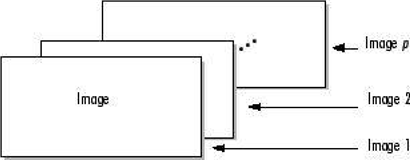
\includegraphics[width=0.6\textwidth]{Imagen25}
\end{center}
\begin{center}
\vskip -0.5cm
\caption{\small{Secuencia de Imágenes.}}
{\small{Fuente: Elaboración propia.}}
\end{center}
\end{figure}

\subsection{Características:}
Cada archivo de una secuencia de imágenes representa un fotograma de vídeo. Así que por ejemplo en 30 segundos de clip, con 30 cuadros por segundo, se tendría 900 archivos de imagen. Aunque las secuencias de imágenes pueden ser difíciles de trabajar con (debido al volumen de cizalla de archivos), se puede hacer casi cualquier cosa.
\vskip 0.1cm
Las secuencias de imágenes utilizan la misma variedad de formatos de archivo que los archivos de imágenes fijas. Entre algunos de los formatos más utilizados para guardar secuencias de imágenes se encuentran SGI, BMP, JPEG, TIFF y TGA. Mostramos unas pequeñas características de cada una de estas:
\vskip 0.1cm \cite{Web}.

{\bf BMP (Bitmap = Mapa de bits)} \vskip 0.1cm

\begin{itemize}
\item[•] Ha sido muy utilizado porque fue desarrollado para aplicaciones Windows.
\item[•] La imagen se forma mediante una parrilla de píxeles.
\item[•] El formato BMP no sufre pérdidas de calidad y por tanto resulta adecuado para guardar imágenes que se desean manipular posteriormente.
\item[•] Ventaja: Guarda gran cantidad de información de la imagen. 
\item[•] Inconveniente: El archivo tiene un tamaño muy grande.
\end{itemize}

{\bf GIF (Graphics Interchange Format = Formato de Intercambio Gráfico)} \vskip 0.1cm

\begin{itemize}
\item[•] Ha sido diseñado específicamente para comprimir imágenes digitales.
\item[•] Reduce la paleta de colores a 256 colores como máximo (profundidad de color de 8 bits).
\item[•] Admite gamas de menor número de colores y esto permite optimizar el tamaño del archivo que contiene la imagen.
\item[•] Ventaja: Es un formato idóneo para publicar dibujos en la web.
\item[•] Inconveniente: No es recomendable para fotografías de cierta calidad ni originales ya que el color real o verdadero utiliza una paleta de más de 256 colores.
\end{itemize}

{\bf JPG-JPEG (Joint Photographic Experts Group = Grupo de Expertos Fotográficos Unidos)} \vskip 0.1cm

\begin{itemize}
\item[•] Admite una paleta de hasta 16 millones de colores.
\item[•] Es el formato más común junto con el GIF para publicar imágenes en la web.
\item[•] La compresión JPEG puede suponer cierta pérdida de calidad en la imagen. En la mayoría de los casos esta pérdida se puede asumir porque permite reducir el tamaño del archivo y su visualización es aceptable.
\item[•] Ventaja: Es ideal para publicar fotografías en la web siempre y cuando se configuren adecuadamente dimensiones y compresión.
\item[•] Inconveniente: Si se define un factor de compresión se pierde calidad. Por este motivo no es recomendable para archivar originales.
\end{itemize}

{\bf TIF-TIFF (Tagged Image File Format = Formato de Archivo de Imagen Etiquetada)} \vskip 0.1cm

\begin{itemize}
\item[•] Almacena imágenes de una calidad excelente.
\item[•] Utiliza cualquier profundidad de color de 1 a 32 bits.
\item[•] Es el formato ideal para editar o imprimir una imagen.
\item[•] Ventaja: Es ideal para archivar archivos originales.
\item[•] Inconveniente: Produce archivos muy grandes.
\end{itemize}

{\bf PNG (Portable Network Graphic = Gráfico portable para la red)} \skip 0.1cm

\begin{itemize}
\item[•] Es un formato de reciente difusión alternativo al GIF.
\item[•] Tiene una tasa de compresión superior al formato GIF (+10\%)
\item[•] Admite la posibilidad de emplear un número de colores superior a los 256 que impone el GIF.
\item[•] Debido a su reciente aparición sólo es soportado en navegadores modernos como IE 4 o superior.
\end{itemize}

Al igual que los formatos de imagen fija, muchos de estos formatos de secuencias de imágenes admite canales alfa. El nombre de cualquier secuencia de imágenes importada debe contener tres o más dígitos de relleno; por ejemplo, “nombre{\_}imagen.0001.tif”

A las secuencias dinámicas de imágenes se le conocen también como vídeos digitales, se puede definir el vídeo digital como un archivo de datos informáticos con una serie de imágenes en movimiento que pueden contener distintos formatos , cada uno se corresponde con una extensión específica del archivo que lo contiene. Existen muchos tipos de formatos de video. Asimismo cada tipo de archivo admite en cada momento un códec de compresión distinto. Aquí se citan algunos de los más utilizados: 

{\bf AVI (Audio Video Interleaved = Audio y Video Intercalado)} \vskip 0.1cm

\begin{itemize}
\item[•] Es el formato estándar para almacenar vídeo digital. Cuando se captura vídeo desde una cámara digital al ordenador, se suele almacenar en este formato con el códec DV (Digital Video).
\item[•] El archivo AVI puede contener vídeo con una calidad excelente. Sin embargo el peso del archivo resulta siempre muy elevado.
\end{itemize}

{\bf MPEG (Moving Pictures Expert Group = Grupo de Expertos de Películas)} \vskip 0.1cm

\begin{itemize}
\item[•] Es un formato estándar para la compresión de video digital.
\item[•] Son archivos de extensión *.MPG ó *.MPEG.
\item[•] Admite distintos tipos de códecs de compresión: MPEG-1 (calidad CD), MPEG-2 (calidad DVD), MPEG-3 (orientado al audio MP3) y MPEG-4 (más orientado a la web).
\end{itemize}

{\bf FLV} \vskip 0.1cm

\begin{itemize}
\item[•] Es un formato que utiliza el reproductor Adobe Flash para visualizar vídeo en Internet.
\item[•] Utiliza el códec Sorenson Spark y el códec On2 VP6.
\item[•] Ambos permiten una alta calidad visual con bitrates reducidos.
\item[•] Son archivos de extensión *.FLV.
\item[•] Opción recomendada para la web por su accesibilidad.
\end{itemize}

\chapter{Desarrollo}

En el presente capítulo, se realiza  el diseño del agente inteligente, para eso primero veremos la estructura del agente y para cada fase del procesamiento haremos comparaciones de varios algoritmos para seleccionar los más adecuados para el reconocimiento de expresiones faciales.

\section{Estructura del Agente}
\subsection{PEAS}
Primero vamos a realizar un análisis del entorno con el PEAS del agente visto en el capítulo anterior (sección 2.2.2) 

\begin{table}[ht!]
\centering
\caption{PEAS Reconocimiento de expresiones faciales.} \vskip 0.1cm
\begin{tabular}{|p{2.7cm} |p{3cm} |p{3.8cm} |p{2cm} |p{2.1cm}|}  \hline 
\bf Tipo de Agente & \bf Performance & \bf Entorno & \bf Actuadores & \bf Sensores \\ \hline 
Reconocedor de expresiones faciales & Reconocimiento correcto de expresiones faciales & Entorno controlado de personas naturales frente a la cámara & Pantalla del monitor & Cámara web \\ \hline
\end{tabular} 
\begin{center}
{\small{Fuente: Elaboración propia.}}
\end{center}
\end{table}

\subsection{Tipo de agente}
La clasificación de nuestro agente según los conceptos abordados en el capítulo anterior (sección 2.2.4)  la podemos expresar de la siguiente manera:

\begin{itemize}
\item[•] Según su tipo: Reflejos simples
\item[•] Según su taxonomía: Agente Reactivo
\item[•] Según su función: Monitorización
\end{itemize}

\subsection{Función del agente}
Teniendo en cuenta el tipo de agente proponemos la siguiente función para el agente inteligente, representada en la tabla x.
\vskip 0.1cm
F(X): X: Secuencia de imágenes con expresiones faciales.

\begin{table}[ht!]
\centering
\caption{Función del agente inteligente.} \vskip 0.1cm
\begin{tabular}{|p{4cm} |p{3.5cm}|}  \hline 
\bf Percepción & \bf Acción \\ \hline 
Secuencia de imágenes con expresiones faciales. & Reconoce expresión facial. \\ \hline
\end{tabular} 
\begin{center}
{\small{Fuente: Elaboración propia.}}
\end{center}
\end{table}

\subsection{Programa del agente}
El programa se encarga de descomponer la secuencia de imágenes y analizar cada una para realizar el proceso de visión computacional para poder reconocer las expresiones faciales y poder mostrar luego los resultados en pantalla. Los pasos de visión computacional son:

\begin{itemize}
\item[•] Preprocesamiento
\item[•] Segmentación
\item[•] Descripción
\item[•] Reconocimiento e interpretación
\end{itemize}

\subsection{Diseño del agente inteligente}
Teniendo en cuenta todos los elementos vistos en los puntos anteriores podemos proseguir con el diseño de nuestro agente inteligente, el cual mediante el sensor (cámara) percibe las secuencias dinámicas de imágenes con expresiones faciales y las evalúa según los pasos de visión artificial y muestra en la pantalla del actuador (computador) la expresión reconocida. para una mejor visualización podemos observar la figura 3.1.

\begin{figure}[ht]
\begin{center}
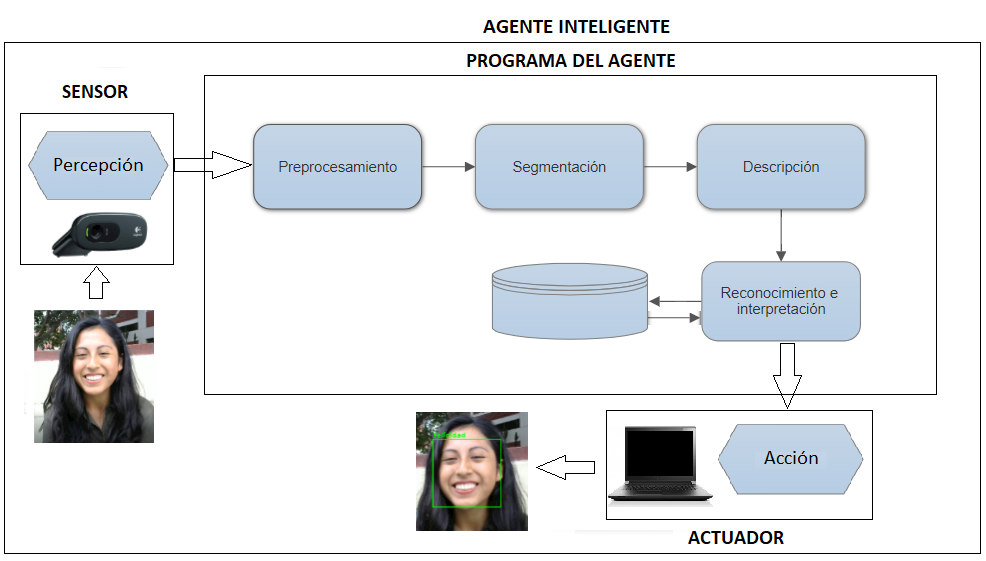
\includegraphics[width=1\textwidth]{Imagen26}
\end{center}
\begin{center}
\vskip -0.5cm
\caption{\small{Agente inteligente.}}
{\small{Fuente: Elaboración propia.}}
\end{center}
\end{figure}

\vskip 3cm

\section{Clasificación de algoritmos}
En cada etapa del diseño vamos a ver distintos criterios que usaremos para evaluar tanto en la parte de las cámaras como los algoritmos del programa del agente. El criterio de evaluación para los procesos a continuación está basado en una escala del 0
al 5.

\begin{table}[ht!]
\centering
\caption{Escala de evaluación.} \vskip 0.1cm
\begin{tabular}{|c|c|c|c|c|c|c|} \hline
\bf 0 & \bf 1 & \bf 2 & \bf 3 & \bf 4 & \bf 5 \\ \hline
No aplica & Malo & Regular & Normal & Bueno & Muy bueno \\ \hline 
\end{tabular}
\begin{center}
{\small{Fuente: Elaboración propia.}}
\end{center}
\end{table}
\vskip 3cm

\begin{itemize}
\item[•] {\bf Arquitectura:} \vskip 0.1cm
{\bf Sensores} \vskip 0.1cm
La percepción del entorno se hace a través de una cámara web, en la sección 2.4.1 vemos distintos tipos de cámaras y los criterios que vamos a evaluar, esto lo podemos expresar en la siguiente tabla:

\begin{table}[h!]
\centering
\caption{Cuadro comparativo de cámaras.} \vskip 0.1cm
\begin{tabular}{|p{4.5cm} |p{2.8cm} |p{2.5cm} |p{2.5cm}|} \hline

Algoritmo \par \vskip 0.4cm Criterio & Microsoft LifeCam HD-3000 & Hd Logitech C270 & Genius FaceCam 1000X \\ \hline

Resolución de video & 4 & 4 & 4 \\ \hline 
Frames por segundo (fps) & 5 & 5 & 5 \\ \hline 
Resolución de imagen & 1 & 4 & 3 \\ \hline 
Zoom digital & 5 & 5 & 3 \\ \hline 
{\bf Total} & 16 & 18 & 15 \\ \hline 

\end{tabular}
\begin{center}
{\small{Fuente: Elaboración propia.}}
\end{center}
\end{table}

De acuerdo a los resultados de la comparación decidimos utilizar la cámara web {\bf Hd Logitech C270.}
\vskip 0.1cm
{\bf Actuadores:} \vskip 0.1cm
La salida se mostrará en pantalla del monitor de la computadora del agente, indicando si fue reconocido la expresión facial.

\item[•] {\bf Programa del agente:} \vskip 0.1cm
Las etapas del procesos de visión computacional que vamos a aplicar sobre  las secuencias de imágenes presentadas en la sección 2.4, se presentan a continuación, por cada una de estas etapas compararemos distintos algoritmos para escoger el más adecuado para el reconocimiento.

\begin{enumerate}
{\bf \item Pre procesamiento de la imagen:} \vskip 0.1cm

\begin{enumerate}
{\bf \item[1.1.] Técnicas de realce:} \vskip 0.1cm

\begin{table}[h!]
\centering
\begin{tabular}{|p{4.8cm} |p{2.3cm} |p{3cm} |p{2cm}|} \hline

Algoritmo \par \vskip 0.4cm Criterio & Ampliación del contraste & Ecualización por histograma & Filtro paso alto \\ \hline

Complejidad computacional & 2 & 3 & 3 \\ \hline 
Distribución uniforme de niveles de gris & 3 & 4 & 3 \\ \hline 
Procesamiento puntual & 2 & 4 & 2 \\ \hline 
{\bf Total} & 7 & 11 & 8 \\ \hline 

\end{tabular}
\end{table}

En base a los resultados obtenidos, la técnica de realce de contraste que se debería emplear es la de filtro paso alto. 

{\bf \item[1.2.] Técnicas de reducción de ruido mediante filtros:} \vskip 0.1cm

\begin{table}[h!]
\centering
\begin{tabular}{|p{4.4cm} |p{3.4cm} |p{2.3cm} |p{2cm}|} \hline

Algoritmo \par \vskip 0.4cm Criterio & Apertura (Erosión, Dilatación) & Filtro de la mediana & Filtro Gaussiano \\ \hline

Reduce ruido impulsivo & 2 & 2 & 4 \\ \hline 
Preservar bordes & 3 & 3 & 2 \\ \hline 
Suavizado uniforme & 3 & 2 & 4 \\ \hline 
{\bf Total} & 8 & 7 & 10 \\ \hline 

\end{tabular}
\end{table}

En base a los resultados obtenidos, la técnica de reducción de ruido que se debería emplear es el filtro gaussiano.
\end{enumerate}

{\bf \item Segmentación:}

\begin{table}[h!]
\centering
\begin{tabular}{|p{4.4cm} |p{1.5cm} |p{3.7cm} |} \hline

Descriptor \par \vskip 0.4cm Criterio & HAAR & HOG (Histograma de gradiente orientado) \\ \hline

Invarianza con la translación, rotación y escalado & 4 & 3 \\ \hline 
Facilidad de búsqueda de patrones & 4 & 4 \\ \hline 
Tiempo de procesamiento & 2 & 4 \\ \hline 
{\bf Total} & 10 & 11 \\ \hline 

\end{tabular}
\end{table}

En base a los resultados obtenidos, el descriptor para obtener el rostro que se debería emplear es el descriptor HOG.

{\bf \item Descripción:}

\begin{table}[h!]
\centering
\begin{tabular}{|p{4.7cm} |p{4.3cm} |p{2.5cm} |p{1.3cm}|} \hline

Algoritmo \par \vskip 0.4cm Criterio & Análisis de componentes independientes (ICA) & Patrón binario local (LBP) & Filtro Gabor \\ \hline

Complejidad computacional & 2 & 4 & 3 \\ \hline 
Sensibilidad a cambios de tamaño, rotación, traslación & 3 & 3 & 3 \\ \hline 
Cantidad de píxeles en el objeto & 3 & 4 & 3 \\ \hline 
{\bf Total} & 8 & 11 & 9 \\ \hline 

\end{tabular}
\end{table}

En base a los resultados obtenidos, la técnica de descripción que se debería emplear es Patrón binario local (LBP).

\vskip 3cm

{\bf \item Reconocimiento e interpretación:}

\begin{table}[h!]
\centering
\begin{tabular}{|p{4.5cm} |p{2.8cm} |p{3.5cm} |p{3cm}|} \hline

Algoritmo \par \vskip 0.4cm Criterio & Redes Neuronales & Máquinas de Vector Soporte (SVM) & k vecinos más próximos (KNN) \\ \hline

Tasa de reconocimiento & 4 & 5 & 3 \\ \hline 
Eficiencia reconocimiento & 3 & 4 & 3 \\ \hline 
{\bf Total} & 7 & 9 & 6 \\ \hline 

\end{tabular}
\end{table}

\end{enumerate}
\end{itemize}


\chapter{Resultados de la tesis}

\section{Resultados Teóricos}

Secuencia dinámica de imágenes:
\vskip 0.1cm	
Por cada segundo se obtienen 30 frames, cada expresión es tomada durante dos segundos, por lo que  se analiza un frame de cada 5 frames, obteniendo en total 12 frames por expresión, y un total de 72 frames por video analizado.  

\begin{figure}[ht]
\begin{center}
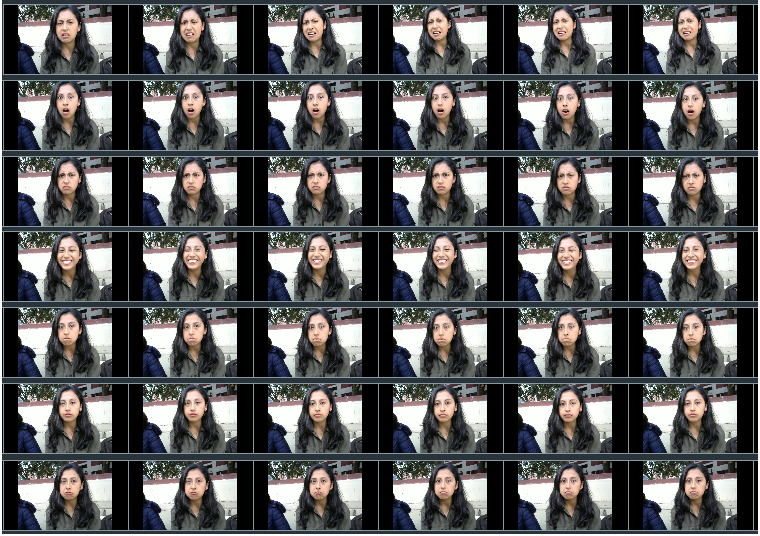
\includegraphics[width=0.9\textwidth]{Imagen27}
\end{center}
\begin{center}
\vskip -0.5cm
\caption{\small{Secuencia dinámica de imágenes.}}
{\small{Fuente: Elaboración propia.}}
\end{center}
\end{figure}

\vskip 7cm
\begin{itemize}
\item[•] Imagen Rostro (facial): \vskip 0.1cm
Recortamos un rostro teniendo en cuento los puntos de referencia faciales, como:

\begin{itemize}
\item Ojos
\item Cejas
\item Nariz
\item Boca
\item Mandíbula
\end{itemize}

\begin{figure}[ht]
\begin{center}
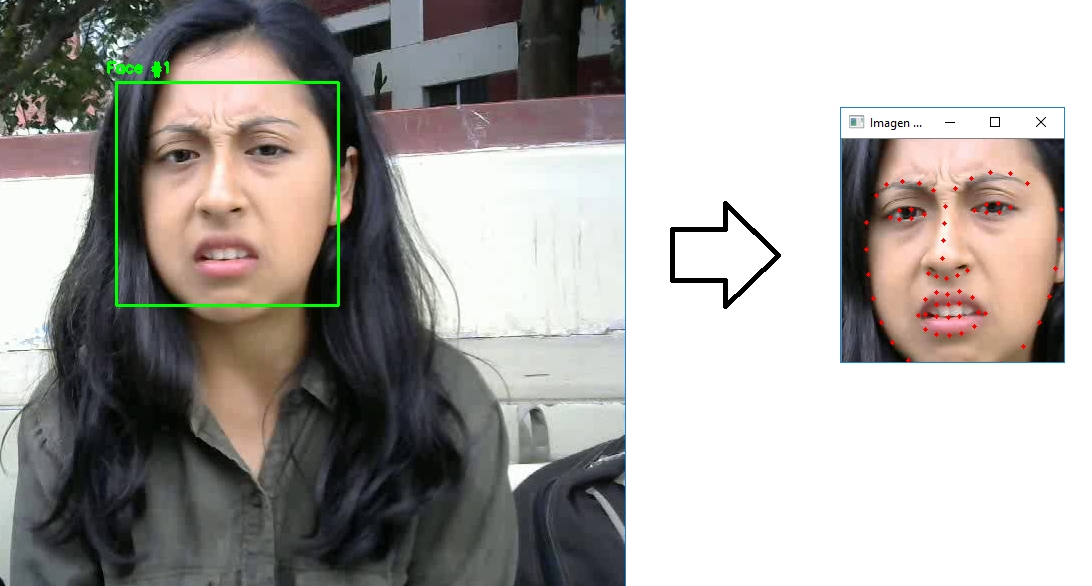
\includegraphics[width=0.45\textwidth]{Imagen28}
\end{center}
\begin{center}
\vskip -0.5cm
\caption{\small{Rostro Detectado y recortado manteniendo sus componentes.}}
{\small{Fuente: Elaboración propia.}}
\end{center}
\end{figure}

\item[•] Expresión facial: \vskip 0.1cm
La expresión facial es la forma que toma el rostro según la forma de sus componentes, así como podemos observar en la siguiente imagen:

\begin{figure}[ht]
\begin{center}
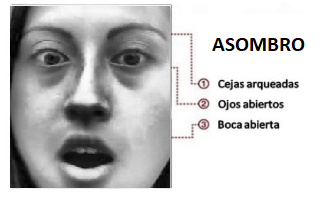
\includegraphics[width=0.4\textwidth]{Imagen29}
\end{center}
\begin{center}
\vskip -0.5cm
\caption{\small{Forma de la expresión facial.}}
{\small{Fuente: Elaboración propia.}}
\end{center}
\end{figure}

Tipos de expresiones faciales: \vskip 0.1cm
Según \cite{Ekman} son 6 expresiones básicas universales más un estado que es considerado neutro.

\begin{figure}[ht]
\begin{center}
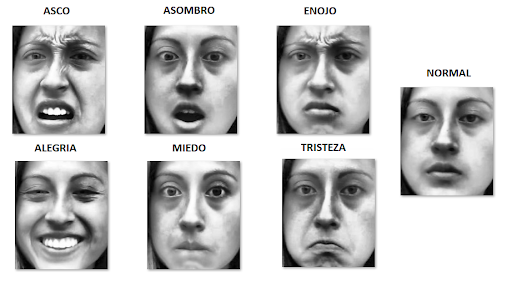
\includegraphics[width=0.8\textwidth]{Imagen30}
\end{center}
\begin{center}
\vskip -0.5cm
\caption{\small{Falta título aquí.}}
{\small{Fuente: Elaboración propia.}}
\end{center}
\end{figure}

\begin{figure}[ht]
\begin{center}
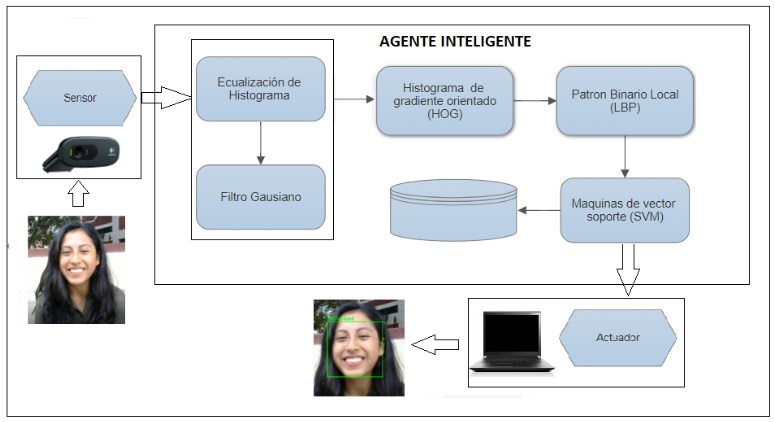
\includegraphics[width=1\textwidth]{Imagen31}
\end{center}
\begin{center}
\vskip -0.5cm
\caption{\small{Estructura del agente con los algoritmos seleccionados.}}
{\small{Fuente: Elaboración propia.}}
\end{center}
\end{figure}

\end{itemize}

\vskip 7cm

\section{Resultados Experimentales}

A continuación, se presentarán los resultados obtenidos por el agente inteligente desarrollado en base a los algoritmos determinados en el capítulo III. Dichos algoritmos fueron implementados con el lenguaje de programación Python y su ejecución se realizó en una computadora con sistema operativo Windows 10, procesador Intel Core i5-3770 y 8 GB de memoria RAM. \vskip 0.1cm

{\bf Análisis de indicadores:} \vskip 0.1cm
Para verificar el funcionamiento del agente inteligente se realizaron experimentos con 70 videos que contenían 7 expresiones faciales, estos videos fueron grabados en ambientes controlados bajo criterio personal.
\vskip 0.1cm
Para demostrar el funcionamiento del agente inteligente utilizamos el modelo de la matriz de confusión por clases la cual analizaremos por cada clase e iremos formando un modelo de matriz de confusión (tabla MC) por cada clase (Expresión facial).

\begin{table}[ht!]
\centering
\caption{Matriz de confusión} \vskip 0.1cm
\begin{tabular}{|c|c|c|c|} \hline
 & Expresión \par & Expresión \par \\
& reconocida & mal reconocida\\ \hline
Expresión \par & \bf VP & \bf FN \\ 
correcta & & \\ \hline 
Expresión \par & \bf FP & \bf VN \\ 
incorrecta & & \\ \hline 
\end{tabular}
\begin{center}
{\small{Fuente: Elaboración propia.}}
\end{center}
\end{table}

Donde: \vskip 0.1cm

\begin{itemize}
\item[•] VP: son los casos que pertenecen a la clase y el clasificador los definió en esa clase. 
\item[•] FN: son los casos que sí pertenecen a la clase y el clasificador no los definió en esa clase. 
\item[•] FP: son los casos que no pertenecen a la clase pero el clasificador los definió en esa clase. 
\item[•] VN: son los casos que no pertenecen a la clase y el clasificador definió que no pertenecen a esa clase.
\end{itemize}

\vskip 5cm
Clase Asco:

\begin{table}[ht!]
\centering
\begin{tabular}{|c|c|c|c|c|c|c|c|c|} \hline
 & \bf Asco & \bf Asombro & \bf Enojo & \bf Felicidad & \bf Miedo & \bf Normal & \bf Tristeza \\ \hline
\bf Asco & 63 & 2 & 0 & 2 & 1 & 2 & 0 \\ \hline
\bf Asombro & 0 & 68 & 0 & 0 & 0 & 1 & 1 \\ \hline
\bf Enojo & 0 & 0 & 66 & 1 & 0 & 3 & 0 \\ \hline
\bf Felicidad & 0 & 0 & 0 & 70 & 0 & 0 & 0 \\ \hline
\bf Miedo & 4 & 0 & 0 & 1 & 55 & 6 & 4 \\ \hline
\bf Normal & 0 & 0 & 0 & 2 & 0 & 68 & 0 \\ \hline
\bf Tristeza & 0 & 0 & 0 & 0 & 1 & 2 & 67 \\ \hline

\end{tabular}
\end{table}


\begin{table}[ht!]
\centering
\begin{tabular}{|c|c|c|} \hline
\bf 63 \par & \bf 7 \par \\
\bf VP & \bf FN \\ \hline
\bf 4 \par & \bf 416 \par \\ 
\bf FP & \bf VN \\ \hline 
\end{tabular}
\end{table}

\begin{equation}
Sensibilidad=S=\frac{VP}{VP+FN}x100=\frac{63}{63+7}=90\%
\end{equation}

\begin{equation}
Especificidad=P=\frac{VN}{VN+FP}x100=\frac{416}{416+4}=99.05\%
\end{equation}

\begin{equation}
Precisi\acute{o}n=E=\frac{VP}{VP+FP}x100=\frac{63}{63+4}x100=94.03\%
\end{equation}

\vskip 5cm

Clase Asombro:

\begin{table}[ht!]
\centering
\begin{tabular}{|c|c|c|c|c|c|c|c|c|} \hline
 & \bf Asco & \bf Asombro & \bf Enojo & \bf Felicidad & \bf Miedo & \bf Normal & \bf Tristeza \\ \hline
\bf Asco & 63 & 2 & 0 & 2 & 1 & 2 & 0 \\ \hline
\bf Asombro & 0 & 68 & 0 & 0 & 0 & 1 & 1 \\ \hline
\bf Enojo & 0 & 0 & 66 & 1 & 0 & 3 & 0 \\ \hline
\bf Felicidad & 0 & 0 & 0 & 70 & 0 & 0 & 0 \\ \hline
\bf Miedo & 4 & 0 & 0 & 1 & 55 & 6 & 4 \\ \hline
\bf Normal & 0 & 0 & 0 & 2 & 0 & 68 & 0 \\ \hline
\bf Tristeza & 0 & 0 & 0 & 0 & 1 & 2 & 67 \\ \hline

\end{tabular}
\end{table}

\begin{table}[ht!]
\centering
\begin{tabular}{|c|c|c|} \hline
\bf 68 \par & \bf 2 \par \\
\bf VP & \bf FN \\ \hline
\bf 2 \par & \bf 418 \par \\ 
\bf FP & \bf VN \\ \hline 
\end{tabular}
\end{table}

\begin{equation}
Sensibilidad=S=\frac{VP}{VP+FN}x100=\frac{68}{68+2}=97.14\%
\end{equation}

\begin{equation}
Especificidad=P=\frac{VN}{VN+FP}x100=\frac{418}{418+2}=99.52\%
\end{equation}

\begin{equation}
Precisi\acute{o}n=E=\frac{VP}{VP+FP}x100=\frac{68}{68+2}x100=97.14\%
\end{equation}

\vskip 5cm

Clase Enojo:

\begin{table}[ht!]
\centering
\caption{Matriz de confusión Múltiple de la clase enojo.} \vskip 0.1cm
\begin{tabular}{|c|c|c|c|c|c|c|c|c|} \hline
 & \bf Asco & \bf Asombro & \bf Enojo & \bf Felicidad & \bf Miedo & \bf Normal & \bf Tristeza \\ \hline
\bf Asco & 63 & 2 & 0 & 2 & 1 & 2 & 0 \\ \hline
\bf Asombro & 0 & 68 & 0 & 0 & 0 & 1 & 1 \\ \hline
\bf Enojo & 0 & 0 & 66 & 1 & 0 & 3 & 0 \\ \hline
\bf Felicidad & 0 & 0 & 0 & 70 & 0 & 0 & 0 \\ \hline
\bf Miedo & 4 & 0 & 0 & 1 & 55 & 6 & 4 \\ \hline
\bf Normal & 0 & 0 & 0 & 2 & 0 & 68 & 0 \\ \hline
\bf Tristeza & 0 & 0 & 0 & 0 & 1 & 2 & 67 \\ \hline

\end{tabular}
\begin{center}
{\small{Fuente: Elaboración propia.}}
\end{center}
\end{table}

\begin{table}[ht!]
\centering
\caption{Matriz de confusión de la clase enojo.} \vskip 0.1cm
\begin{tabular}{|c|c|c|} \hline
\bf 66 \par & \bf 4 \par \\
\bf VP & \bf FN \\ \hline
\bf 0 \par & \bf 420 \par \\ 
\bf FP & \bf VN \\ \hline 
\end{tabular}
\begin{center}
{\small{Fuente: Elaboración propia.}}
\end{center}
\end{table}

\begin{equation}
Sensibilidad=S=\frac{VP}{VP+FN}x100=\frac{66}{66+4}=94.29\%
\end{equation}

\begin{equation}
Especificidad=P=\frac{VN}{VN+FP}x100=\frac{420}{420+0}=100\%
\end{equation}

\begin{equation}
Precisi\acute{o}n=E=\frac{VP}{VP+FP}x100=\frac{66}{66+0}x100=100\%
\end{equation}

\vskip 5cm

Clase Felicidad:

\begin{table}[ht!]
\centering
\caption{Matriz de confusión Múltiple de la clase felicidad.} \vskip 0.1cm
\begin{tabular}{|c|c|c|c|c|c|c|c|c|} \hline
 & \bf Asco & \bf Asombro & \bf Enojo & \bf Felicidad & \bf Miedo & \bf Normal & \bf Tristeza \\ \hline
\bf Asco & 63 & 2 & 0 & 2 & 1 & 2 & 0 \\ \hline
\bf Asombro & 0 & 68 & 0 & 0 & 0 & 1 & 1 \\ \hline
\bf Enojo & 0 & 0 & 66 & 1 & 0 & 3 & 0 \\ \hline
\bf Felicidad & 0 & 0 & 0 & 70 & 0 & 0 & 0 \\ \hline
\bf Miedo & 4 & 0 & 0 & 1 & 55 & 6 & 4 \\ \hline
\bf Normal & 0 & 0 & 0 & 2 & 0 & 68 & 0 \\ \hline
\bf Tristeza & 0 & 0 & 0 & 0 & 1 & 2 & 67 \\ \hline

\end{tabular}
\begin{center}
{\small{Fuente: Elaboración propia.}}
\end{center}
\end{table}

\begin{table}[ht!]
\centering
\caption{Matriz de confusión de la clase felicidad.} \vskip 0.1cm
\begin{tabular}{|c|c|c|} \hline
\bf 70 \par & \bf 0 \par \\
\bf VP & \bf FN \\ \hline
\bf 6 \par & \bf 414 \par \\ 
\bf FP & \bf VN \\ \hline 
\end{tabular}
\begin{center}
{\small{Fuente: Elaboración propia.}}
\end{center}
\end{table}

\begin{equation}
Sensibilidad=S=\frac{VP}{VP+FN}x100=\frac{70}{70+0}=100\%
\end{equation}

\begin{equation}
Especificidad=P=\frac{VN}{VN+FP}x100=\frac{414}{414+6}=98.57\%
\end{equation}

\begin{equation}
Precisi\acute{o}n=E=\frac{VP}{VP+FP}x100=\frac{70}{70+6}x100=92.11\%
\end{equation}

\vskip 5cm

Clase Miedo:

\begin{table}[ht!]
\centering
\caption{Matriz de confusión Múltiple de la clase miedo.} \vskip 0.1cm
\begin{tabular}{|c|c|c|c|c|c|c|c|c|} \hline
 & \bf Asco & \bf Asombro & \bf Enojo & \bf Felicidad & \bf Miedo & \bf Normal & \bf Tristeza \\ \hline
\bf Asco & 63 & 2 & 0 & 2 & 1 & 2 & 0 \\ \hline
\bf Asombro & 0 & 68 & 0 & 0 & 0 & 1 & 1 \\ \hline
\bf Enojo & 0 & 0 & 66 & 1 & 0 & 3 & 0 \\ \hline
\bf Felicidad & 0 & 0 & 0 & 70 & 0 & 0 & 0 \\ \hline
\bf Miedo & 4 & 0 & 0 & 1 & 55 & 6 & 4 \\ \hline
\bf Normal & 0 & 0 & 0 & 2 & 0 & 68 & 0 \\ \hline
\bf Tristeza & 0 & 0 & 0 & 0 & 1 & 2 & 67 \\ \hline

\end{tabular}
\begin{center}
{\small{Fuente: Elaboración propia.}}
\end{center}
\end{table}

\begin{table}[ht!]
\centering
\caption{Matriz de confusión de la clase miedo.} \vskip 0.1cm
\begin{tabular}{|c|c|c|} \hline
\bf 55 \par & \bf 15 \par \\
\bf VP & \bf FN \\ \hline
\bf 2 \par & \bf 418 \par \\ 
\bf FP & \bf VN \\ \hline 
\end{tabular}
\begin{center}
{\small{Fuente: Elaboración propia.}}
\end{center}
\end{table}

\begin{equation}
Sensibilidad=S=\frac{VP}{VP+FN}x100=\frac{55}{55+15}=78.57\%
\end{equation}

\begin{equation}
Especificidad=P=\frac{VN}{VN+FP}x100=\frac{418}{418+2}=99.52\%
\end{equation}

\begin{equation}
Precisi\acute{o}n=E=\frac{VP}{VP+FP}x100=\frac{55}{55+2}x100=96.49\%
\end{equation}

\vskip 5cm

Clase Normal:

\begin{table}[ht!]
\centering
\caption{Matriz de confusión Múltiple de la clase normal.} \vskip 0.1cm
\begin{tabular}{|c|c|c|c|c|c|c|c|c|} \hline
 & \bf Asco & \bf Asombro & \bf Enojo & \bf Felicidad & \bf Miedo & \bf Normal & \bf Tristeza \\ \hline
\bf Asco & 63 & 2 & 0 & 2 & 1 & 2 & 0 \\ \hline
\bf Asombro & 0 & 68 & 0 & 0 & 0 & 1 & 1 \\ \hline
\bf Enojo & 0 & 0 & 66 & 1 & 0 & 3 & 0 \\ \hline
\bf Felicidad & 0 & 0 & 0 & 70 & 0 & 0 & 0 \\ \hline
\bf Miedo & 4 & 0 & 0 & 1 & 55 & 6 & 4 \\ \hline
\bf Normal & 0 & 0 & 0 & 2 & 0 & 68 & 0 \\ \hline
\bf Tristeza & 0 & 0 & 0 & 0 & 1 & 2 & 67 \\ \hline

\end{tabular}
\begin{center}
{\small{Fuente: Elaboración propia.}}
\end{center}
\end{table}

\begin{table}[ht!]
\centering
\caption{Matriz de confusión de la clase normal.} \vskip 0.1cm
\begin{tabular}{|c|c|c|} \hline
\bf 68 \par & \bf 2 \par \\
\bf VP & \bf FN \\ \hline
\bf 14 \par & \bf 406 \par \\ 
\bf FP & \bf VN \\ \hline 
\end{tabular}
\begin{center}
{\small{Fuente: Elaboración propia.}}
\end{center}
\end{table}

\begin{equation}
Sensibilidad=S=\frac{VP}{VP+FN}x100=\frac{68}{68+2}=97.14\%
\end{equation}

\begin{equation}
Especificidad=P=\frac{VN}{VN+FP}x100=\frac{406}{406+14}=96.67\%
\end{equation}

\begin{equation}
Precisi\acute{o}n=E=\frac{VP}{VP+FP}x100=\frac{68}{68+14}x100=82.93\%
\end{equation}

\vskip 5cm

Clase Tristeza:

\begin{table}[ht!]
\centering
\caption{Matriz de confusión Múltiple de la clase tristeza.} \vskip 0.1cm
\begin{tabular}{|c|c|c|c|c|c|c|c|c|} \hline
 & \bf Asco & \bf Asombro & \bf Enojo & \bf Felicidad & \bf Miedo & \bf Normal & \bf Tristeza \\ \hline
\bf Asco & 63 & 2 & 0 & 2 & 1 & 2 & 0 \\ \hline
\bf Asombro & 0 & 68 & 0 & 0 & 0 & 1 & 1 \\ \hline
\bf Enojo & 0 & 0 & 66 & 1 & 0 & 3 & 0 \\ \hline
\bf Felicidad & 0 & 0 & 0 & 70 & 0 & 0 & 0 \\ \hline
\bf Miedo & 4 & 0 & 0 & 1 & 55 & 6 & 4 \\ \hline
\bf Normal & 0 & 0 & 0 & 2 & 0 & 68 & 0 \\ \hline
\bf Tristeza & 0 & 0 & 0 & 0 & 1 & 2 & 67 \\ \hline

\end{tabular}
\begin{center}
{\small{Fuente: Elaboración propia.}}
\end{center}
\end{table}

\begin{table}[ht!]
\centering
\caption{Matriz de confusión de la clase tristeza.} \vskip 0.1cm
\begin{tabular}{|c|c|c|} \hline
\bf 67 \par & \bf 3 \par \\
\bf VP & \bf FN \\ \hline
\bf 5 \par & \bf 415 \par \\ 
\bf FP & \bf VN \\ \hline 
\end{tabular}
\begin{center}
{\small{Fuente: Elaboración propia.}}
\end{center}
\end{table}

\begin{equation}
Sensibilidad=S=\frac{VP}{VP+FN}x100=\frac{67}{67+3}=95.71\%
\end{equation}

\begin{equation}
Especificidad=P=\frac{VN}{VN+FP}x100=\frac{415}{415+5}=98.81\%
\end{equation}

\begin{equation}
Precisi\acute{o}n=E=\frac{VP}{VP+FP}x100=\frac{67}{67+5}x100=93.06\%
\end{equation}

\vskip 5cm

{\bf Indicador 1: Sensibilidad} \vskip 0.1cm
Es la proporción de casos positivos que fueron identificados correctamente. La sensibilidad del agente es la suma de todas las sensibilidades resultantes de sensibilidad por clase entre el total de clases, se calcula mediante la siguiente ecuación:

\begin{equation}
Sensibilidad~Total=St=\frac{\sum_{1}^{i}\frac{VPi}{VPi+FNi}x100}{7}=93.26
\end{equation}

donde i es el número de expresiones. 

\begin{table}[ht!]
\centering
\begin{tabular}{|c|c|c|c|c|c|c|c|c|c|} \hline
\bf Expresión & \bf Asco & \bf Asombro & \bf Enojo & \bf Felicidad & \bf Miedo & \bf Normal & \bf Tristeza & \bf Total \\ \hline
\bf Sensibilidad & 90 & 97.14 & 94.29 & 100 & 78.57 & 97.14 & 95.71 & 93.26 \\ \hline

\end{tabular}
\end{table}

\vskip 1cm

{\bf Indicador 2: Especificidad} \vskip 0.1cm
Es la proporción de casos negativos que fueron identificados correctamente. La Especificidad del agente es la suma de todas las especificidades resultantes de cada clase dividida entre el número de clases, se calcula mediante la siguiente ecuación:

\begin{equation}
Especificidad~Total=Pt=\frac{\sum_{1}^{i}\frac{VNi}{VNi+FPi}x100}{7}=98.88
\end{equation}

donde i es el número de expresiones. 

\begin{table}[ht!]
\centering
\begin{tabular}{|c|c|c|c|c|c|c|c|c|c|} \hline
\bf Expresión & \bf Asco & \bf Asombro & \bf Enojo & \bf Felicidad & \bf Miedo & \bf Normal & \bf Tristeza & \bf Total \\ \hline
\bf Especificidad & 99.05 & 99.52 & 100 & 98.57 & 99.52 & 96.67 & 98.81 & 98.88 \\ \hline

\end{tabular}
\end{table}

\vskip 1cm

{\bf Indicador 3: Precisión} \vskip 0.1cm
Es la proporción de los casos predichos positivos que son correctos. La Precisión del agente es la suma de todos los resultados de precisión por clase entre el total de clases, se utiliza la siguiente ecuación para calcularla:

\begin{equation}
Precisi\acute{o}n~Total=Et=\frac{\sum_{1}^{i}\frac{VPi}{VPi+FPi}x100}{7}=93.68
\end{equation}

donde i es el número de expresiones. 

\begin{table}[ht!]
\centering
\begin{tabular}{|c|c|c|c|c|c|c|c|c|c|} \hline
\bf Expresión & \bf Asco & \bf Asombro & \bf Enojo & \bf Felicidad & \bf Miedo & \bf Normal & \bf Tristeza & \bf Total \\ \hline
\bf Precisión & 94.03 & 97.14 & 100 & 92.11 & 96.49 & 82.93 & 93.06 & 93.68 \\ \hline

\end{tabular}
\end{table}

Comparamos la precisión de nuestro agente inteligente con la precisión de nuestros antecedentes: podemos concluir que nuestro agente inteligente tuvo una mayor tasa de reconocimiento de expresiones faciales. 

\begin{figure}[ht]
\begin{center}
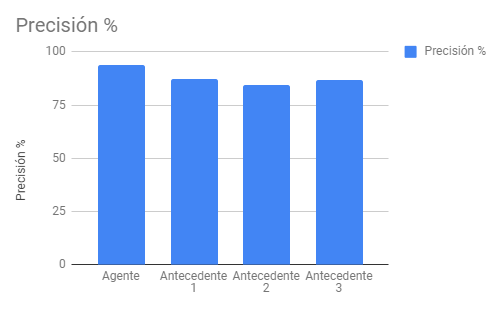
\includegraphics[width=0.45\textwidth]{Imagen32}
\end{center}
\begin{center}
\vskip -0.5cm
\caption{\small{Comparación de Eficacia con Antecedentes.}}
{\small{Fuente: Elaboración propia.}}
\end{center}
\end{figure}

\vskip 3cm

{\bf Para el antecedente 1:} (Precisión = 87.29\%) nuestro agente inteligente obtuvo mayor precisión gracias a la secuencia de imágenes en el entrenamiento, las cuales fueron material propio. 
\vskip 0.1cm

{\bf Para el antecedente 2:} (Precisión = 84.4\%) se obtuvo mayor precisión ya que ellos analizaron 4 expresiones faciales, y nuestro agente inteligente analizó 6 expresiones faciales y se utilizó el algoritmo LBP a vez del PCA para mejor reconocimiento.
\vskip 0.1cm

{\bf Para el antecedente 3:} (Precisión = 86.6\%) se obtuvo mayor precisión ya que ellos analizaron el rostro de perfil, mientras que nosotros analizamos las rostros de frente.

\chapter{Consideraciones finales}

\section{Conclusiones}

Culminando la presente tesis, cuyo objetivo general fue: “Diseñar un agente inteligente que permita reconocer expresiones faciales en secuencia dinámica de imágenes”, el cual fue logrado obteniendo un reconocimiento de 7 expresiones faciales las cuales son: asco, asombro, enojo, felicidad, miedo, normal, tristeza.
\vskip 0.3cm

\begin{itemize}
\item[•] El agente inteligente, es capaz de reconocer las expresiones faciales con una sensibilidad del 93.26\% el cual supera al 90\% trazado en nuestro objetivo específico.
\item[•] Se logró determinar la especificidad del agente, es decir la tasa de verdaderos negativos del 98.88\% el cual supera al 90\% trazado en nuestro objetivo específico, comprobando de esta manera que gracias a un ambiente controlado y a que solo se analizaron videos en las cuales se encontraban solo 7 expresiones a predecir.
\item[•] En secuencia dinámica de imágenes mediante el agente inteligente se logró una precisión del 93.68\% superando a nuestro objetivo inicial del 90\%.
\item[•] Se demostró que el agente inteligente pudo reconocer la expresión facial en un conjunto de expresiones faciales demostrando así la eficacia de mas un 90\%.
\end{itemize}

\section{Trabajos futuros}

\begin{itemize}
\item[-] Evaluar al agente inteligente en lugares con ambientes no controlados donde la secuencia de imágenes no siempre contengan expresiones faciales.
\item[-] Fortalecer al agente inteligente con algoritmos que ayuden a identificar exactamente las expresiones faciales que han obtenido un bajo porcentaje y reconocer más expresiones faciales.
\end{itemize}


